\chapter{Ανάπτυξη Διαδικτυακής Εφαρμογής iBoot}
Σε αυτό το κεφάλαιο, αναλύονται οι λειτουργίες που παρέχει η διαδικτυακή εφαρμογή στους χρήστες της μέσω Διεπαφής Χρήστη (User Interface) και παρέχεται επεξήγηση των αρχείων κώδικα, ο οποίος συντέλεσε στη δημιουργία του πληροφοριακού συστήματος. Ανάλογα με τον ρόλο του χρήστη που συνδέεται στην εφαρμογή, παρέχονται και οι αντίστοιχες λειτουργίες. Η εμφάνιση της εφαρμογής έχει ίδια αισθητικά χαρακτηριστικά για κάθε είδος χρήστη. Το User Interface θεωρείται από τα πιο σημαντικά μέρη μιας διαδικτυακής εφαρμογής καθώς, αν είναι σχεδιασμένο σωστά, ώστε να είναι εύχρηστο και διαισθητικό, κάνει εύκολη τη χρήση των λειτουργιών του συστήματος, ακόμη και σε χρήστες που πιθανώς δεν είναι εξειδικευμένοι στον τομέα της πληροφορικής.

Για την κατασκευή του User Interface, χρησιμοποιήθηκε η αρχή του Reactive Programming, δηλαδή της μεθόδου προγραμματισμού ιστού ώστε το περιεχόμενο της εφαρμογής να ανανεώνεται δυναμικά και ασύγχρονα με τις ενέργειες του χρήστη, σε ένα εν γένει στατικό περιβάλλον. Όσον αφορά το σχεδιασμό του γραφικού περιβάλλοντος, χρησιμοποιήθηκε Responsive Design, ώστε η εφαρμογή να έχει ομοιόμορφη, καλαίσθητη και λειτουργική εμφάνιση, τόσο σε συσκευές με μεγάλη διάμετρο οθόνης, όπως ηλεκτρονικούς υπολογιστές, όσο και σε συσκευές με μικρότερη διάμετρο οθόνης, όπως κινητά τηλέφωνα. Ο συνδυασμός των παραπάνω μεθόδων προγραμματισμού ιστού, προσφέρει ευχάριστη εμπειρία χρήσης της εφαρμογής, σε όλους τους χρήστες, ανεξάρτητα από τον τύπο συσκευής που χρησιμοποιούν.

Η διαδικτυακή εφαρμογή έχει υλοποιηθεί ως ένα γραφικό περιβάλλον ιστού που επικοινωνεί με τη βάση δεδομένων του μέσω ενός RESTful API. Για την ανάπτυξη της εφαρμογής έγινε χρήση του CodeIgniter PHP Framework. Η αναλυτική προδιαγραφή του API που παρέχει η πλατφόρμα, μετά την εγκατάσταση της, δημιουργήθηκε με χρήση του Swagger UI και βρίσκεται στην τοποθεσία \texttt{/api} και περιγράφει όλες τις λειτουργίες που είναι δυνατό να πραγματοποιηθούν με τη χρήση του.

\section{Διεπαφή Χρήστη}

\subsection{Εγγραφή \& Σύνδεση στο Σύστημα}
\FloatBarrier
Η σελίδα εγγραφής στο σύστημα απεικονίζεται στο σχήμα \ref{fig:iBoot_register} και είναι προσβάσιμη στη διεύθυνση \verb!/register!.
\begin{figure}[ht]
	\centering
	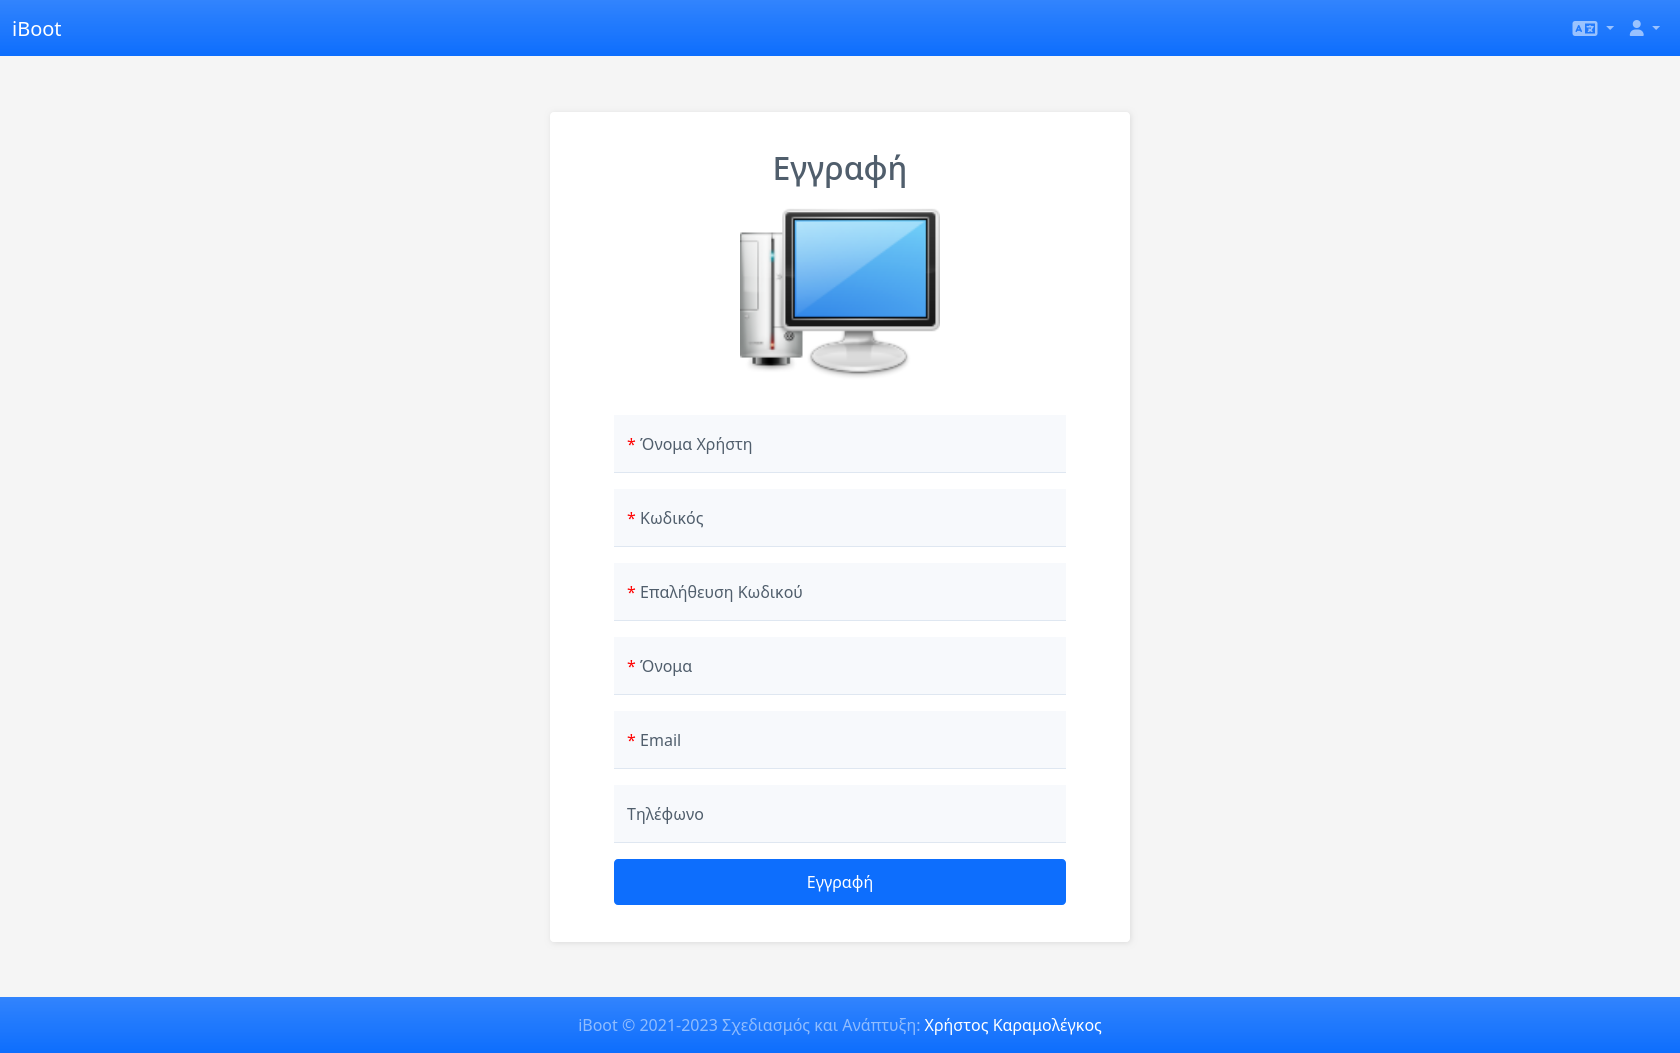
\includegraphics[scale=0.25]{iBoot-register.png}
	\caption{iBoot - Εγγραφή}
	\label{fig:iBoot_register}
\end{figure}

Ο χρήστης θα πρέπει να συμπληρώσει εκεί τα στοιχεία που ζητούνται και στη συνέχεια να πατήσει το κουμπί της εγγραφής για να δημιουργηθεί ο λογαριασμός του. Αν δεν υπάρχει κανένας εγγεγραμμένος διαχειριστής στο σύστημα, η ίδια σελίδα αξιοποιείται για την εγγραφή του. Στη συνέχεια, οι επόμενοι χρήστες που εγγράφονται δεν έχουν ρόλο διαχειριστή. Ο υπάρχων διαχειριστής μπορεί να δώσει ρόλο διαχειριστή σε άλλους χρήστες από τη σελίδα διαχείρισης χρηστών \ref{fig:iBoot_users}.

Η σελίδα σύνδεσης στο σύστημα απεικονίζεται στο σχήμα \ref{fig:iBoot_login} και είναι προσβάσιμη στη διεύθυνση \verb!/login!.
\begin{figure}[ht]
	\centering
	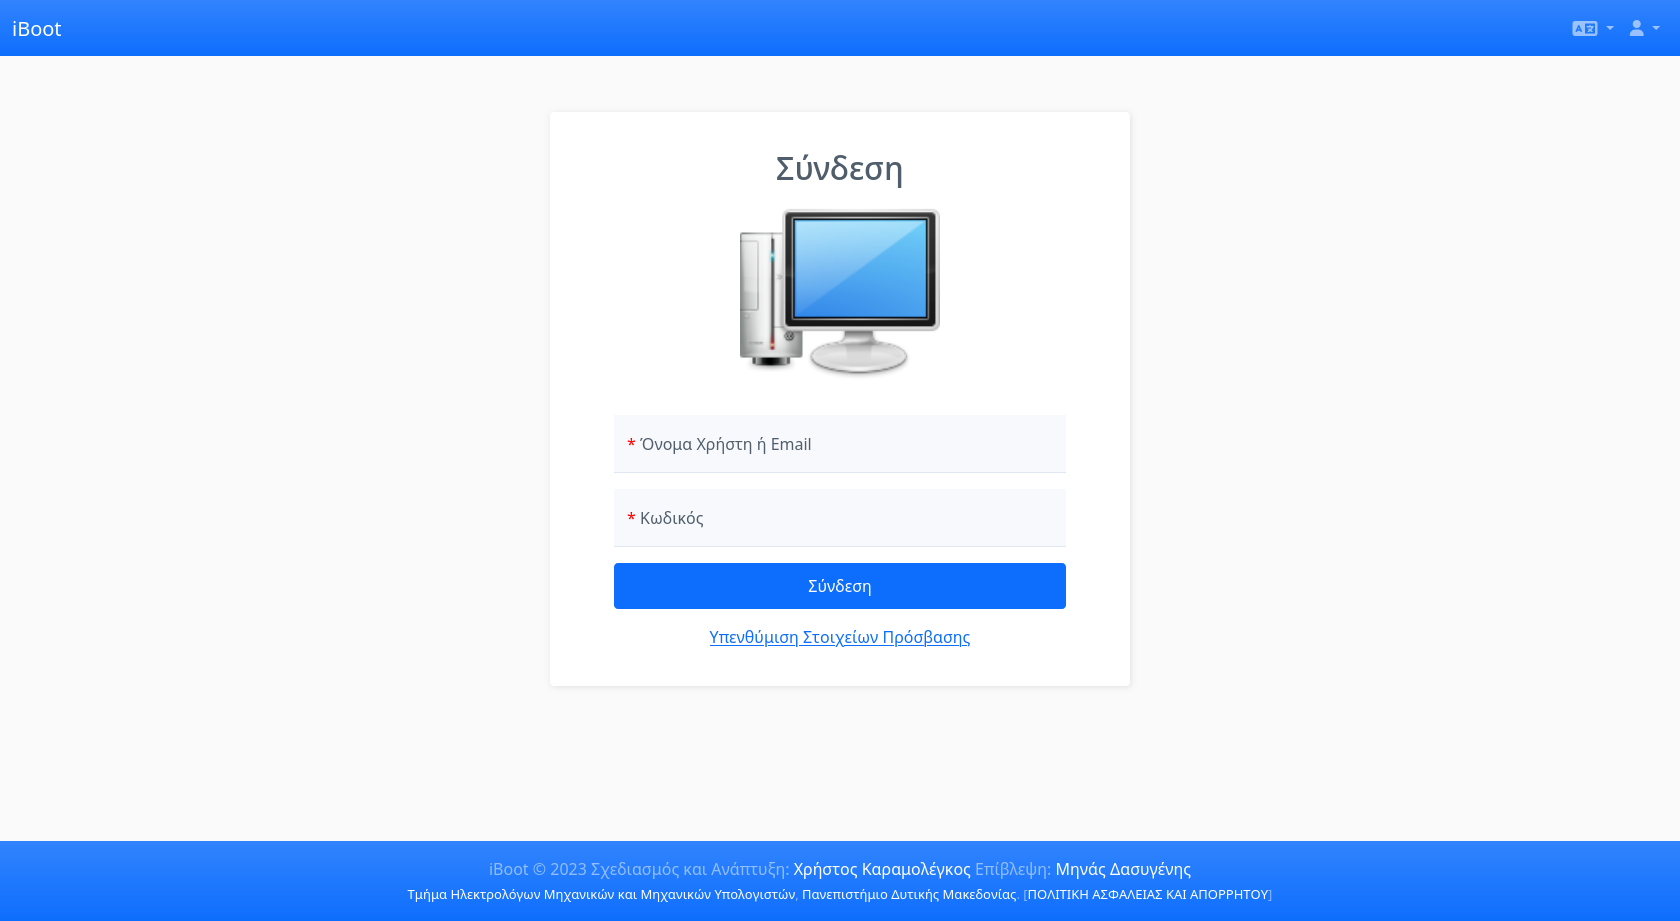
\includegraphics[scale=0.25]{iBoot-login.png}
	\caption{iBoot - Σύνδεση}
	\label{fig:iBoot_login}
\end{figure}

Αν κάποιος χρήστης ξεχάσει τα στοιχεία πρόσβασής του και επιθυμεί να τα αλλάξει, θα πρέπει να επισκευτεί τη διεύθυνση \verb!/forgotCredentials!, η οποία απεικονίζεται στο σχήμα \ref{fig:iBoot_forgot_credentials}. Εκεί, ο χρήστης έχει τη δυνατότητα να αιτηθεί την επανέκδοση του κωδικού πρόσβασής του, με χρήση του ονόματος χρήστη ή του email του. Μετά την υποβολή της φόρμας επανέκδοσης κωδικού πρόσβασης, ο χρήστης θα λάβει ένα email με έναν σύνδεσμο, τον οποίο θα πρέπει να ακολουθήσει για να δηλώσει τον νέο κωδικό πρόσβασής του. Σε περίπτωση που δε θυμάται το όνομα χρήστη του, μπορεί να βάλει το email του στη φόρμα υπενθύμισης ονόματος χρήστη και να λάβει ένα email που να αναφέρει το όνομα χρήστη του.
\begin{figure}[ht]
	\centering
	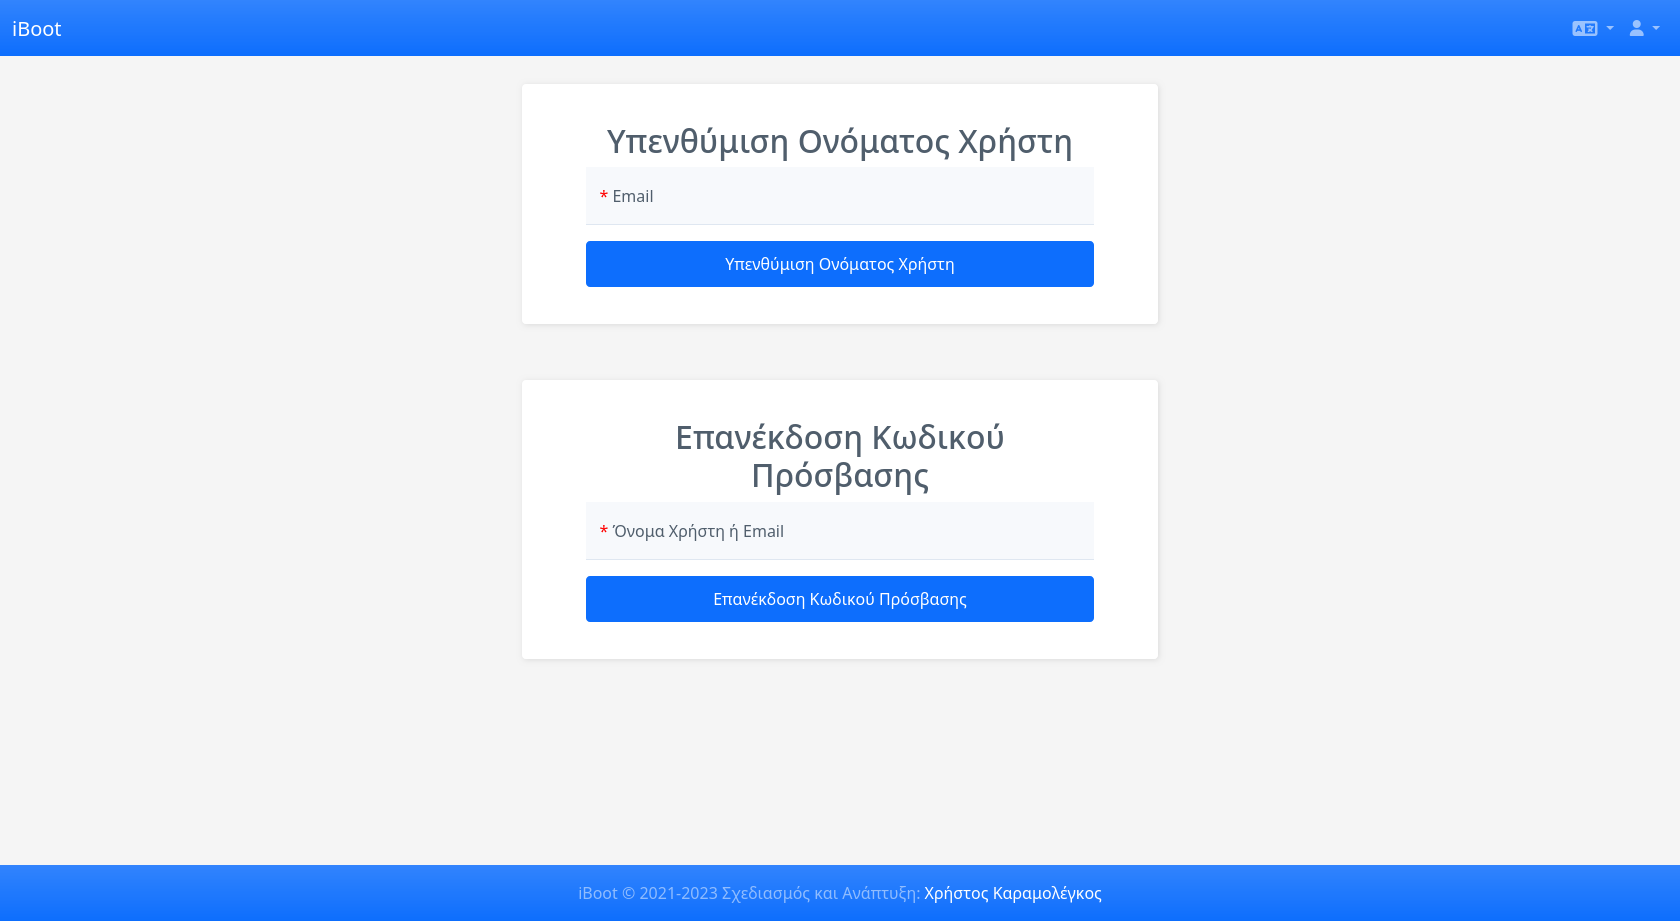
\includegraphics[scale=0.25]{iBoot-forgot_credentials.png}
	\caption{iBoot - Υπενθύμιση Στοιχείων Πρόσβασης}
	\label{fig:iBoot_forgot_credentials}
\end{figure}
\FloatBarrier

\subsection{Αρχική Σελίδα}
\FloatBarrier
Η αρχική σελίδα, προσβάσιμη στη διεύθυνση \verb!/dashboard!, στην οποία μεταφέρεται ο χρήστης μετά τη σύνδεσή του (αν δεν είχε ζητήσει κάποια διαφορετική σελίδα).

Όπως φαίνεται στο σχήμα \ref{fig:iBoot_dashboard}, η αρχική σελίδα περιέχει συνδέσμους προς άλλες σημαντικές σελίδες της εφαρμογής.
\begin{figure}[ht]
	\centering
	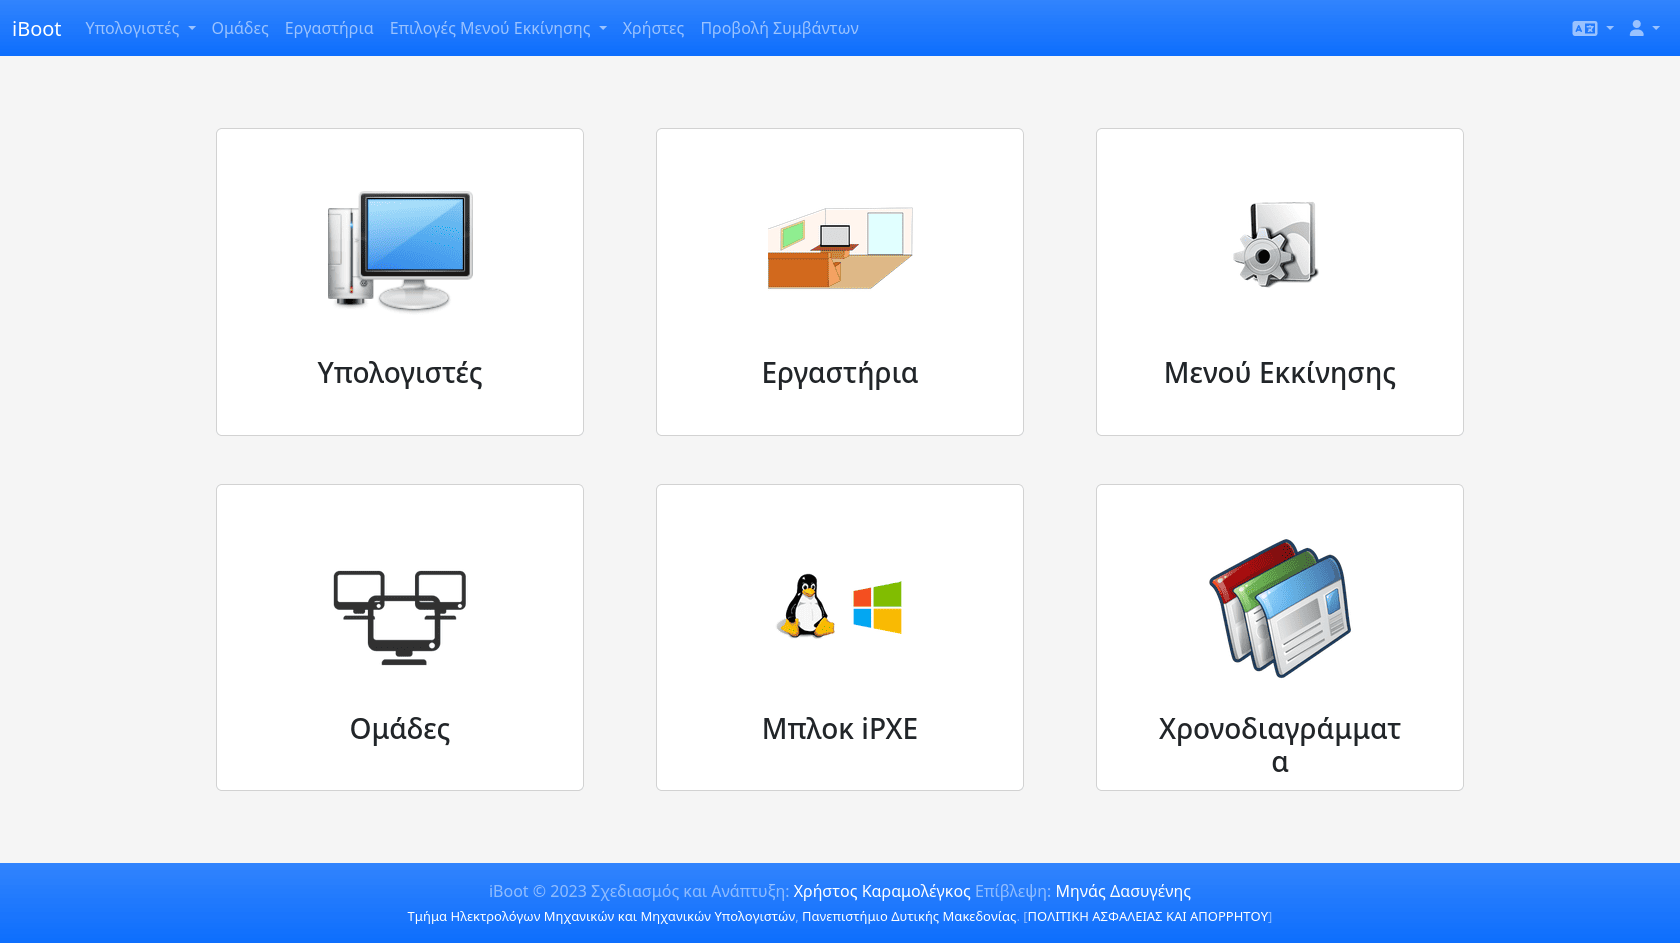
\includegraphics[scale=0.25]{iBoot-dashboard.png}
	\caption{iBoot - Αρχική Σελίδα}
	\label{fig:iBoot_dashboard}
\end{figure}
\FloatBarrier

\subsection{Μενού Πλοήγησης}
\FloatBarrier
Στο σχήμα \ref{fig:iBoot_nav_admin}, απεικονίζεται η μπάρα του μενού πλοήγησης για τους χρήστες με ρόλο διαχειριστή.

Στο αριστερό μέρος της μπάρας υπάρχει το όνομα της εφαρμογής, το οποίο αν πατηθεί επιστρέφει τον χρήστη την αρχική της σελίδα. Αμέσως μετά εμφανίζεται μια σειρά από επιλογές για τις διαθέσιμες στον χρήστη σελίδες.

Η πρώτη επιλογή στο αριστερό μέρος της μπάρας του μενού πλοήγησης, αφορά την απεικόνιση υπολογιστών. Όταν ο χρήστης περιηγηθεί με το ποντίκι του πάνω στην επιλογή (σε υπολογιστή) ή επιλέξει να την επεκτείνει (σε κινητές συσκευές), θα του παρουσιαστούν οι επιλογές απεικόνισης είτε Διαχειριζόμενων (Σχήμα \ref{fig:iBoot_computers}) είτε Μη Εκχωρημένων Υπολογιστών (Σχήμα \ref{fig:iBoot_computers_unassigned}).

Η δεύτερη επιλογή κατευθύνει τον χρήστη στη σελίδα απεικόνισης των Ομάδων υπολογιστών (Σχήμα \ref{fig:iBoot_groups}), ενώ η τρίτη σε αυτή της απεικόνισης των Εργαστηρίων (Σχήμα \ref{fig:iBoot_labs}).

Η επόμενη ομάδα επιλογών, μπορεί να επεκταθεί με πανομοιότυπο τρόπο με την πρώτη, και αφορά την απεικόνιση των Μπλοκ Εντολών τύπου iPXE (Σχήμα \ref{fig:iBoot_ipxeblocks}), των Μενού Εκκίνησης (Σχήμα \ref{fig:iBoot_bootmenu}) και των Χρονοδιαγραμμάτων (Σχήμα \ref{fig:iBoot_schedules}).

Στη συνέχεια, βρίσκεται η επιλογή των Χρηστών της εφαρμογής (Σχήμα \ref{fig:iBoot_users}) και στο τέλος του αριστερού τμήματος της μπάρας πλοήγησης βρίσκεται η επιλογή απεικόνισης των αρχείων καταγραφής συμβάντων (Σχήμα \ref{fig:iBoot_logs}).

Στο δεξί μέρος της μπάρας πλοήγησης υπάρχουν πρώτα ο επιλογέας γλώσσας της εφαρμογής και έπειτα η ομάδα επιλογών της προβολής των στοιχείων του προφίλ του χρήστη και της αποσύνδεσής του.

\begin{figure}[ht]
	\centering
	
\includegraphics[scale=0.25]{iBoot-nav_admin.png}
	\caption{iBoot - Μενού Πλοήγησης Διαχειριστή}
	\label{fig:iBoot_nav_admin}
\end{figure}

Όπως είναι εμφανές στο σχήμα \ref{fig:iBoot_nav_user}, η μπάρα πλοήγησης των χρηστών με ρόλο διαχειριστή εργαστηρίου είναι σχεδόν πανομοιότυπη με εκείνη των χρηστών με ρόλο διαχειριστή. Η διαφορά του βρίσκεται στο ότι από την πρώτη απουσιάζουν οι επιλογές απεικόνισης χρηστών και προβολής των αρχείων καταγραφής συμβάντων, καθώς οι χρήστες που δεν έχουν ρόλο διαχειριστή δεν έχουν και πρόσβαση σε αυτές τις σελίδες.
\begin{figure}[ht]
	\centering
	
\includegraphics[scale=0.25]{iBoot-nav_user.png}
	\caption{iBoot - Μενού Πλοήγησης Διαχειριστή Εργαστηρίου}
	\label{fig:iBoot_nav_user}
\end{figure}

Οι επιλογές του αριστερού τμήματος της μπάρας πλοήγησης απουσιάζουν εντελώς όταν ο χρήστης είναι μη αυθεντικοποιημένος επισκέπτης, όπως φαίνεται στο σχήμα \ref{fig:iBoot_nav_guest}. Εκείνος δηλαδή βλέπει μόνο το όνομα της εφαρμογής στο αριστερό μέρος της μπάρας πλοήγησης και στο δεξί μέρος της τον επιλογέα γλώσσας της εφαρμογής και την ομάδα επιλογών για πραγματοποίηση σύνδεσης και εγγραφής (αν αυτή είναι ενεργοποιημένη ως δυνατότητα του συστήματος).
\begin{figure}[ht]
	\centering
	
\includegraphics[scale=0.25]{iBoot-nav_guest.png}
	\caption{iBoot - Μενού Πλοήγησης Επισκέπτη}
	\label{fig:iBoot_nav_guest}
\end{figure}
\FloatBarrier

\subsection{Υπολογιστές}
\FloatBarrier
Στη σελίδα Διαχειριζόμενων Υπολογιστών, προσβάσιμη στη διεύθυνση \verb!/computers_managed!, ο χρήστης μπορεί να δει τους υπολογιστές των οποίων τα στοιχεία έχει δικαίωμα να διαχειριστεί. Αν ο χρήστης είναι διαχειριστής, βλέπει όλους τους υπολογιστές που έχουν εγγραφεί στην πλατφόρμα. Αν είναι διαχειριστής εργαστηρίου, τότε βλέπει μόνο τους υπολογιστές που βρίσκονται σε εργαστήρια που αυτός διαχειρίζεται.

Όπως φαίνεται στο σχήμα \ref{fig:iBoot_computers}, ο πίνακας με τα στοιχεία των υπολογιστών αποτελείται από τις παρακάτω στήλες:
\begin{itemize}
	\item Υπολογιστής: Το όνομα που έχει δοθεί στον υπολογιστή
	\item UUID: Το μοναδικό αναγνωριστικό UUID του υπολογιστή
	\item MAC: Η φυσική διεύθυνση διεπαφής δικτύου (MAC address) του υπολογιστή
	\item Σημείωση: Πεδίο ελεύθερου κειμένου για διατήρηση σημειώσεων σχετικά με τον υπολογιστή
	\item Ομάδες: Πεδίο πολλαπλής επιλογής, περιέχει τις ομάδες των οποίων είναι μέλος ο υπολογιστής
	\item Εργαστήριο: Πεδίο επιλογής, περιέχει το εργαστήριο στο οποίο βρίσκεται ο υπολογιστής
	\item Τελευταία Εκκίνηση: Χρονοσφραγίδα τελευταίας εκκίνησης του υπολογιστή μέσω του συστήματος.
	\item Διαγραφή: Κουμπί για τη διαγραφή του υπολογιστή από το σύστημα
\end{itemize}

\begin{figure}[ht]
	\centering
	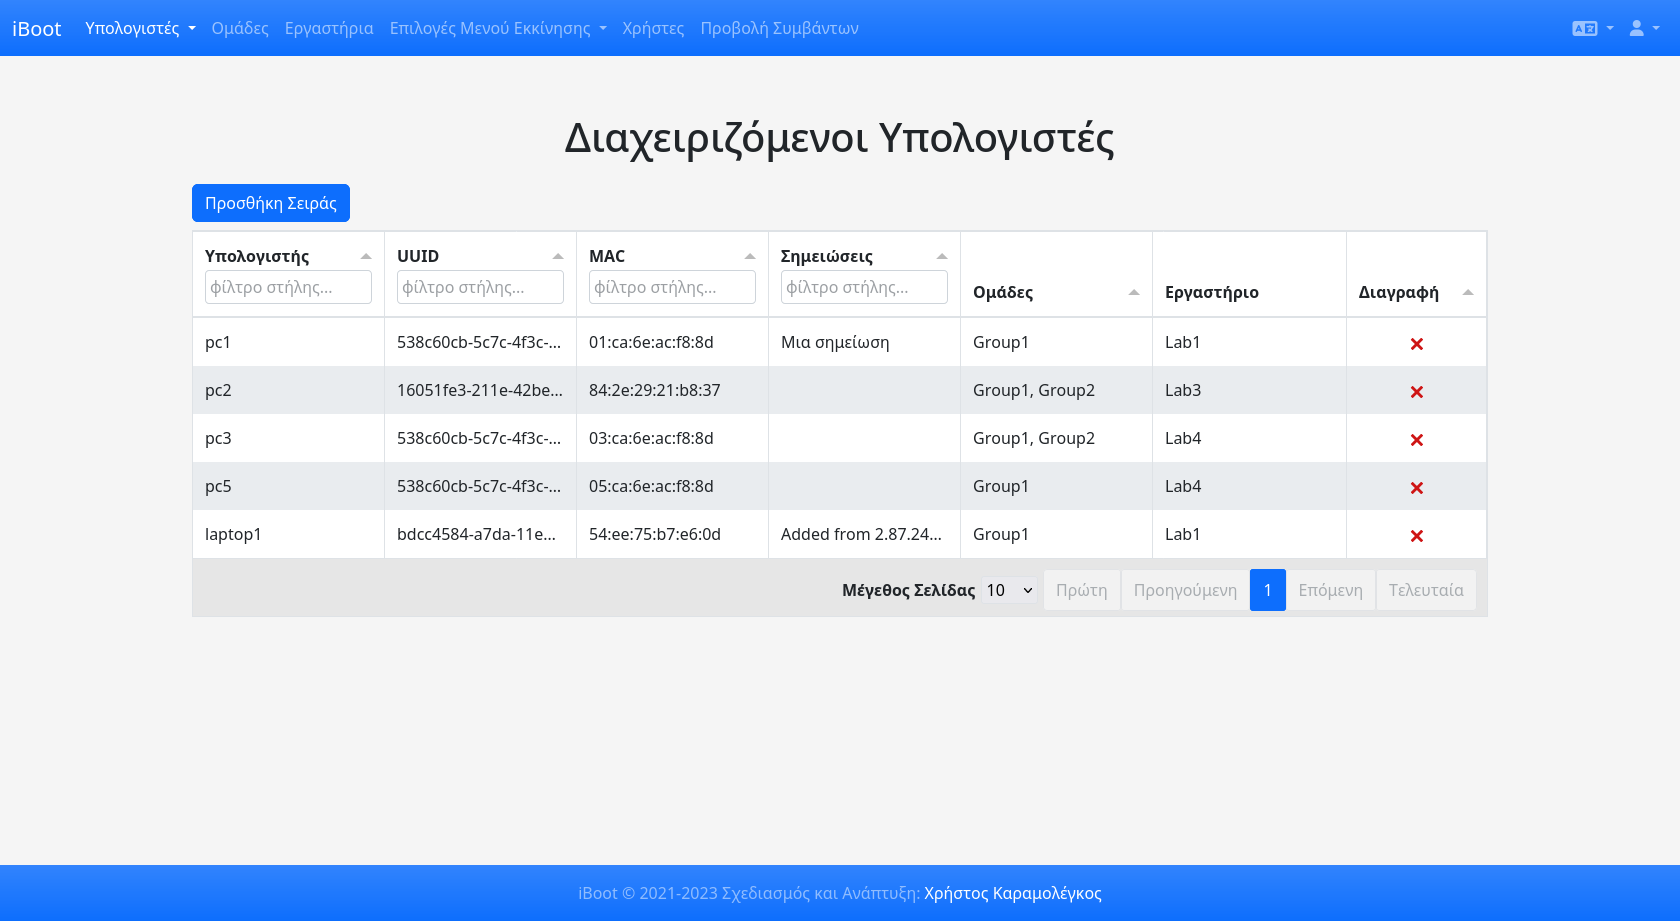
\includegraphics[scale=0.25]{iBoot-computers.png}
	\caption{iBoot - Διαχειριζόμενοι Υπολογιστές}
	\label{fig:iBoot_computers}
\end{figure}
Διαχειριζόμενοι Υπολογιστές θεωρούνται όσοι έχουν τοποθετηθεί σε κάποιο εργαστήριο, από έναν διαχειριστή ή διαχειριστή εργαστηρίου.

Όσοι υπολογιστές είναι εγγεγραμμένοι στο σύστημα αλλά δεν έχουν τοποθετηθεί σε κάποιο εργαστήριο, θεωρούνται Μη Εκχωρημένοι και εμφανίζονται σε ξεχωριστό πίνακα, ο οποίος απεικονίζεται στο σχήμα \ref{fig:iBoot_computers_unassigned} και είναι προσβάσιμος στη διεύθυνση \verb!/computers_unassigned!. Στον πίνακα με τους Μη Εκχωρημένους Υπολογιστές έχουν πρόσβαση όλοι οι χρήστες, ώστε να μπορούν να τοποθετούν τους υπολογιστές σε εργαστήρια, χωρίς ανάγκη παρέμβασης κάποιου διαχειριστή.

\begin{figure}[ht]
	\centering
	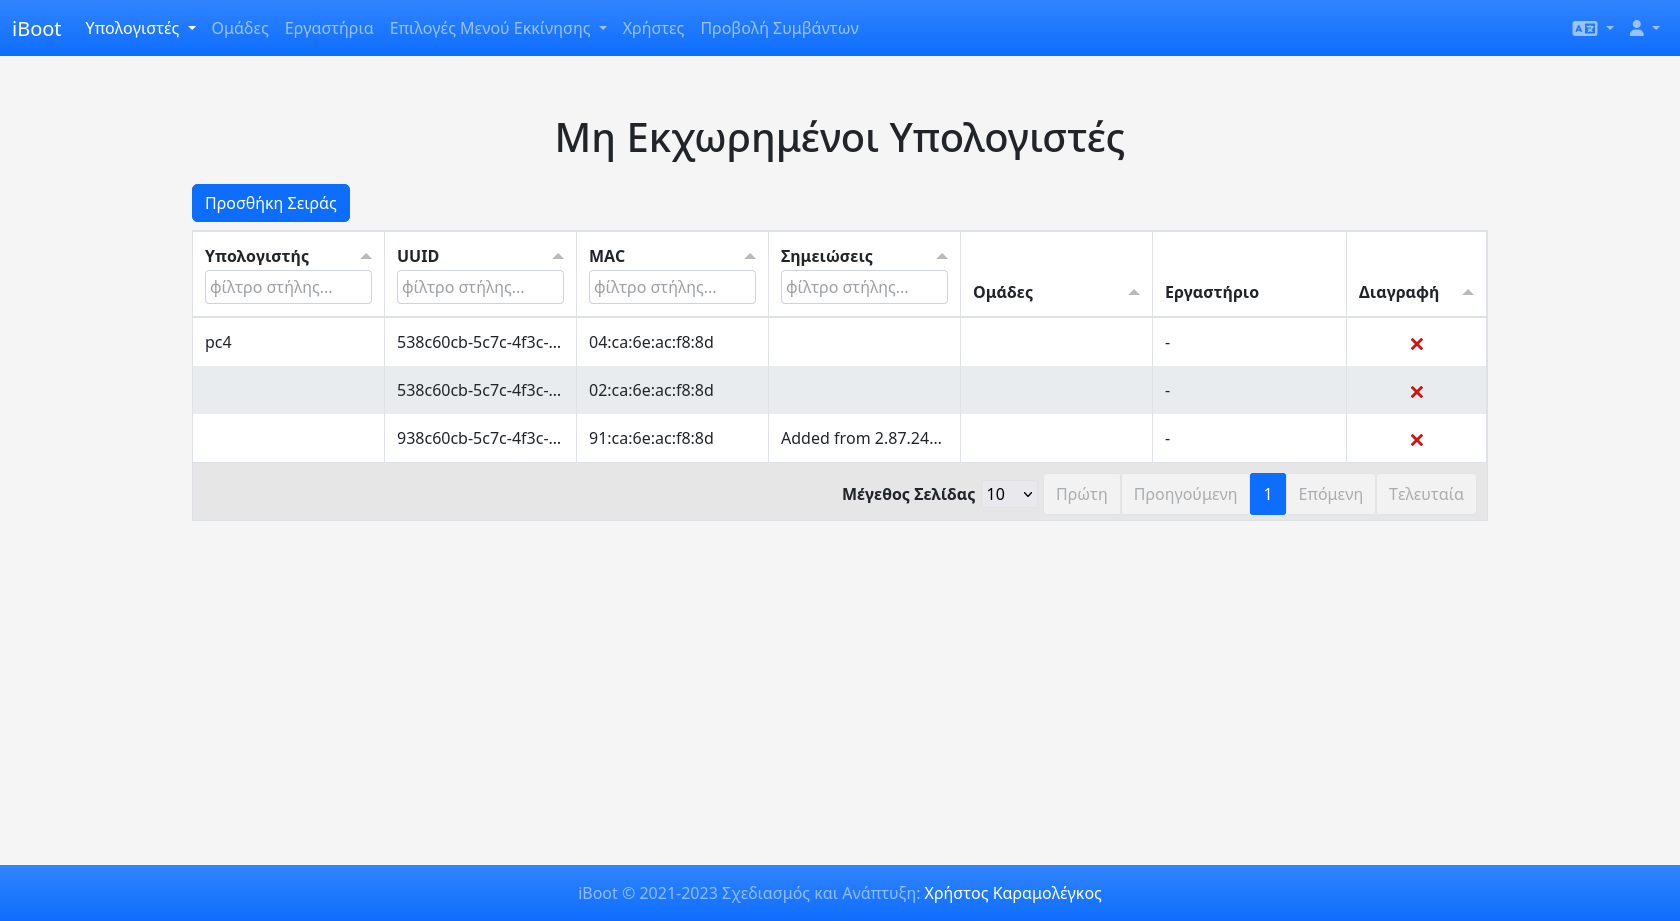
\includegraphics[scale=0.25]{iBoot-computers_unassigned.png}
	\caption{iBoot - Μη Εκχωρημένοι Υπολογιστές}
	\label{fig:iBoot_computers_unassigned}
\end{figure}
\FloatBarrier

Φυσικά, οι διαχειριστές εργαστηρίων μπορούν να τοποθετούν τους υπολογιστές μόνο σε εργαστήρια που οι ίδιοι διαχειρίζονται, ενώ οι διαχειριστές μπορούν να τοποθετούν οποιονδήποτε υπολογιστή σε οποιοδήποτε εργαστήριο, ακόμη και αν κάποιος άλλος χρήστης είχε τοποθετήσει τον υπολογιστή σε άλλο εργαστήριο νωρίτερα. Αντίστοιχα, αν κάποιος αφαιρέσει έναν υπολογιστή από εργαστήριο, τότε αυτός θα εμφανίζεται στον πίνακα των Μη Εκχωρημένων και οποιοσδήποτε θα έχει τη δυνατότητα να τον προσθέσει σε κάποιο εργαστήριο στο οποίο έχει πρόσβαση.

Στις σελίδες που αφορούν τους υπολογιστές, έχει προστεθεί ένα πλαίσιο επιλογής (checkbox) για την ενεργοποίηση και απενεργοποίηση της λειτουργίας αυτόματης επαναφόρτωσης των δεδομένων των υπολογιστών. Αν το πλαίσιο είναι επιλεγμένο, η δυνατότητα επεξεργασίας στοιχείων απενεργοποιείται και κάθε πέντε δευτερόλεπτα γίνεται κλήση AJAX στο endpoint του REST API της εφαρμογής, ώστε ο πίνακας των υπολογιστών να ξαναγεμίζεται με ενημερωμένα δεδομένα. Αυτό, σε συνδυασμό με φίλτρο λεπτών στο πεδίο τηε τελευταίας εκκίνησης, επιτρέπει τη ζωντανή παρακολούθηση της εκκίνησης των υπολογιστών.

\subsection{Ομάδες Υπολογιστών}
\FloatBarrier
Στη σελίδα Ομάδων Υπολογιστών, προσβάσιμη στη διεύθυνση \verb!/groups!, ο χρήστης μπορεί να δει τις ομάδες υπολογιστών που έχουν δημιουργηθεί και τους υπολογιστές που έχουν προστεθεί σε αυτές. Αν ο χρήστης είναι διαχειριστής, βλέπει όλους τους υπολογιστές που έχει μια ομάδα, διαφορετικά μόνο εκείνους που βρίσκονται σε εργαστήρια τα οποία διαχειρίζεται.

Όπως φαίνεται στο σχήμα \ref{fig:iBoot_groups}, ο πίνακας με τα στοιχεία των ομάδων αποτελείται από τις παρακάτω στήλες:
\begin{itemize}
	\item Ομάδα: Το όνομα που έχει δοθεί στην ομάδα
	\item IP διακομιστή: Η διεύθυνση του διακομιστή στον οποίο μπορούν οι υπολογιστές - μέλη της ομάδας να αναζητήσουν εικόνες λειτουργικών συστημάτων
	\item Πρόθεμα διαδρομής διακομιστή: Το πρόθεμα της διαδρομής στον διακομιστή, όπου βρίσκονται οι εικόνες των λειτουργικών συστημάτων
	\item Υπολογιστές: Πεδίο πολλαπλής επιλογής, περιέχει τους υπολογιστές οι οποίοι είναι μέλη της ομάδας
	\item Διαγραφή: Κουμπί για τη διαγραφή της ομάδας από το σύστημα
\end{itemize}

\begin{figure}[ht]
	\centering
	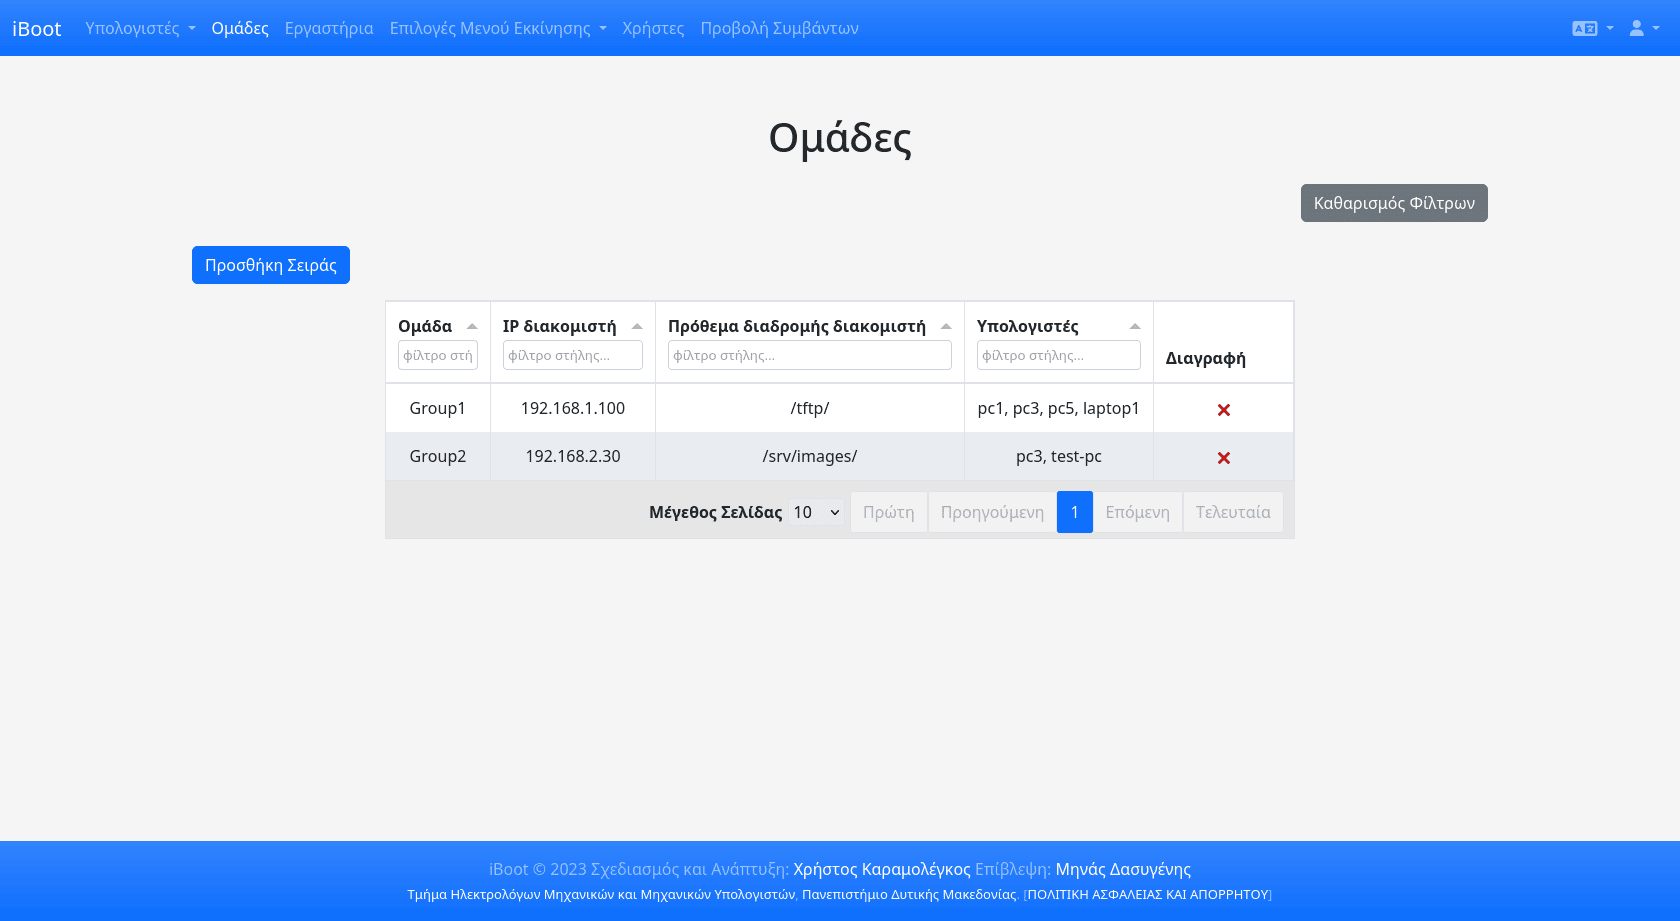
\includegraphics[scale=0.25]{iBoot-groups.png}
	\caption{iBoot - Διαχείριση Ομάδων Υπολογιστών}
	\label{fig:iBoot_groups}
\end{figure}

Τα πεδία \emph{IP διακομιστή} και \emph{Πρόθεμα διαδρομής διακομιστή} μπορούν να χρησιμοποιηθούν μέσω των προκαθορισμένων μεταβλητών \emph{\$\{group.ip\}} και \emph{\$\{group.prefix\}} αντίστοιχα, σε καταχωρήσεις μενού iPXE.
\FloatBarrier

\subsection{Εργαστήρια}
\FloatBarrier
Στη σελίδα των Εργαστηρίων, προσβάσιμη στη διεύθυνση \verb!/labs!, ο χρήστης μπορεί να δει τα στοιχεία των εργαστηρίων που έχουν δημιουργηθεί.

Όπως φαίνεται στο σχήμα \ref{fig:iBoot_labs}, ο πίνακας με τα στοιχεία των εργαστηρίων αποτελείται από τις παρακάτω στήλες:
\begin{itemize}
	\item Εργαστήριο: Το όνομα που έχει δοθεί στο εργαστήριο
	\item Διεύθυνση: Η διεύθυνση του εργαστηρίου
	\item Τηλέφωνο: Το τηλέφωνο του εργαστηρίου, αν έχει προστεθεί
	\item Διαγραφή: Κουμπί για τη διαγραφή του εργαστηρίου από το σύστημα
\end{itemize}
\begin{figure}[ht]
	\centering
	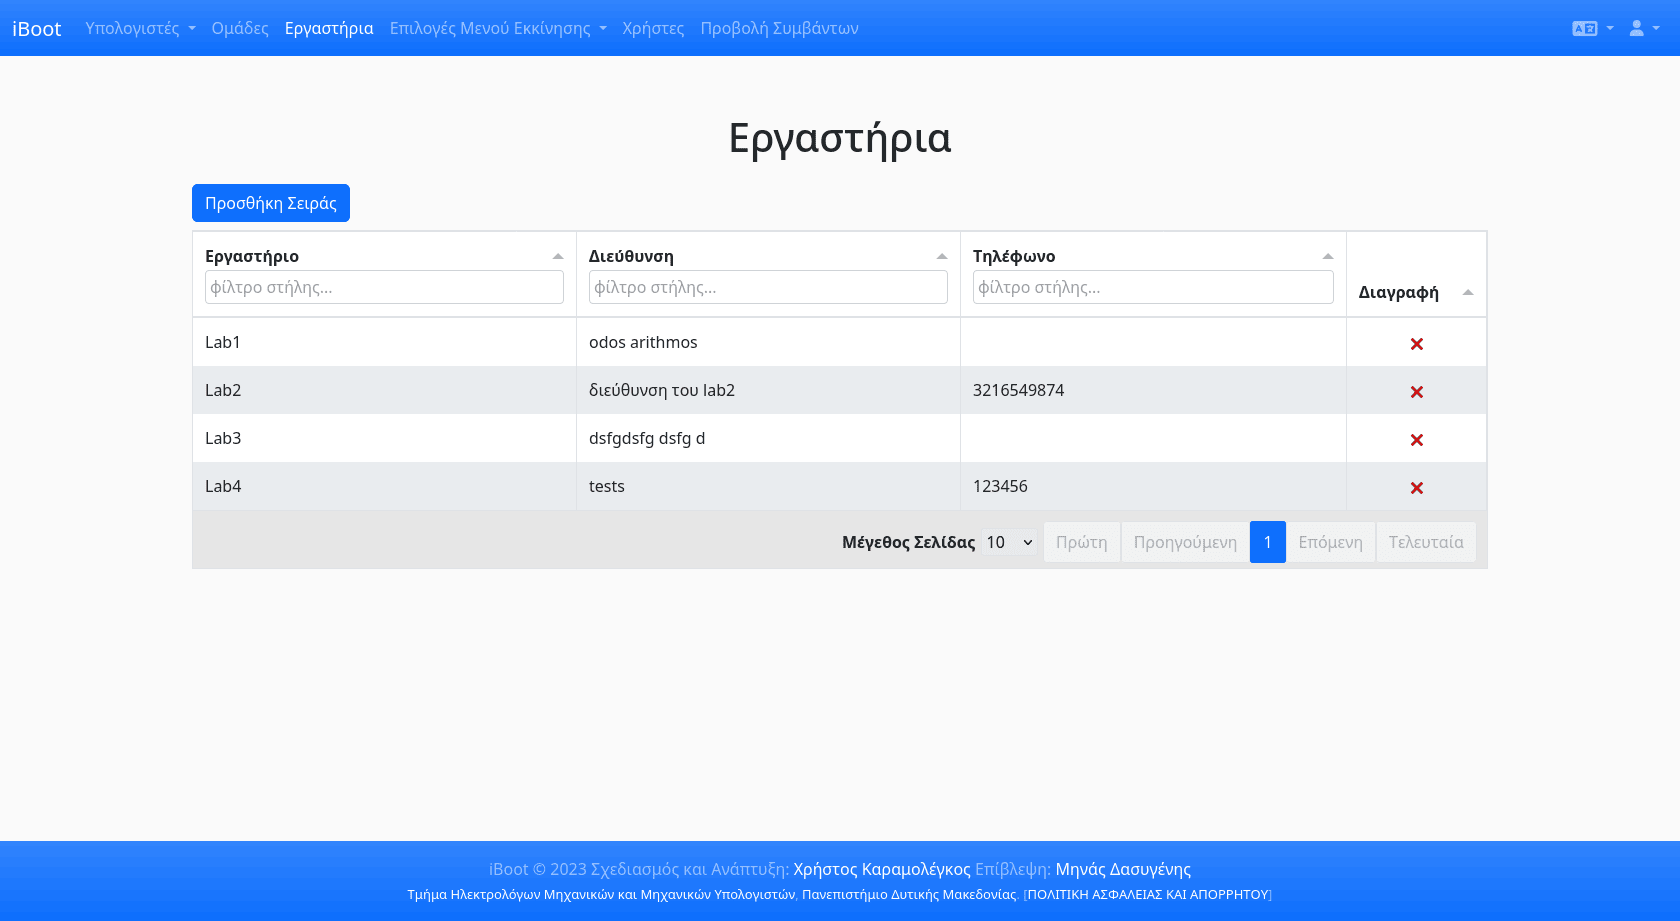
\includegraphics[scale=0.25]{iBoot-labs.png}
	\caption{iBoot - Διαχείριση Εργαστηρίων}
	\label{fig:iBoot_labs}
\end{figure}
\FloatBarrier

\subsection{Block εντολών τύπου iPXE}
\FloatBarrier
Στη σελίδα των Μπλοκ iPXE, προσβάσιμη στη διεύθυνση \verb!/ipxeblocks!, ο χρήστης μπορεί να δει τα στοιχεία των Μπλοκ iPXE που έχουν δημιουργηθεί.

Όπως φαίνεται στο σχήμα \ref{fig:iBoot_ipxeblocks}, ο πίνακας με τα στοιχεία των Μπλοκ iPXE αποτελείται από τις παρακάτω στήλες:
\begin{itemize}
	\item Μπλοκ iPXE: Το όνομα που έχει δοθεί στο Μπλοκ iPXE
	\item Καταχώρηση Μενού iPXE: Το περιεχόμενο της καταχώρησης μπλοκ iPXE
	\item Διαγραφή: Κουμπί για τη διαγραφή του Μπλοκ iPXE από το σύστημα
\end{itemize}

\begin{figure}[ht]
	\centering
	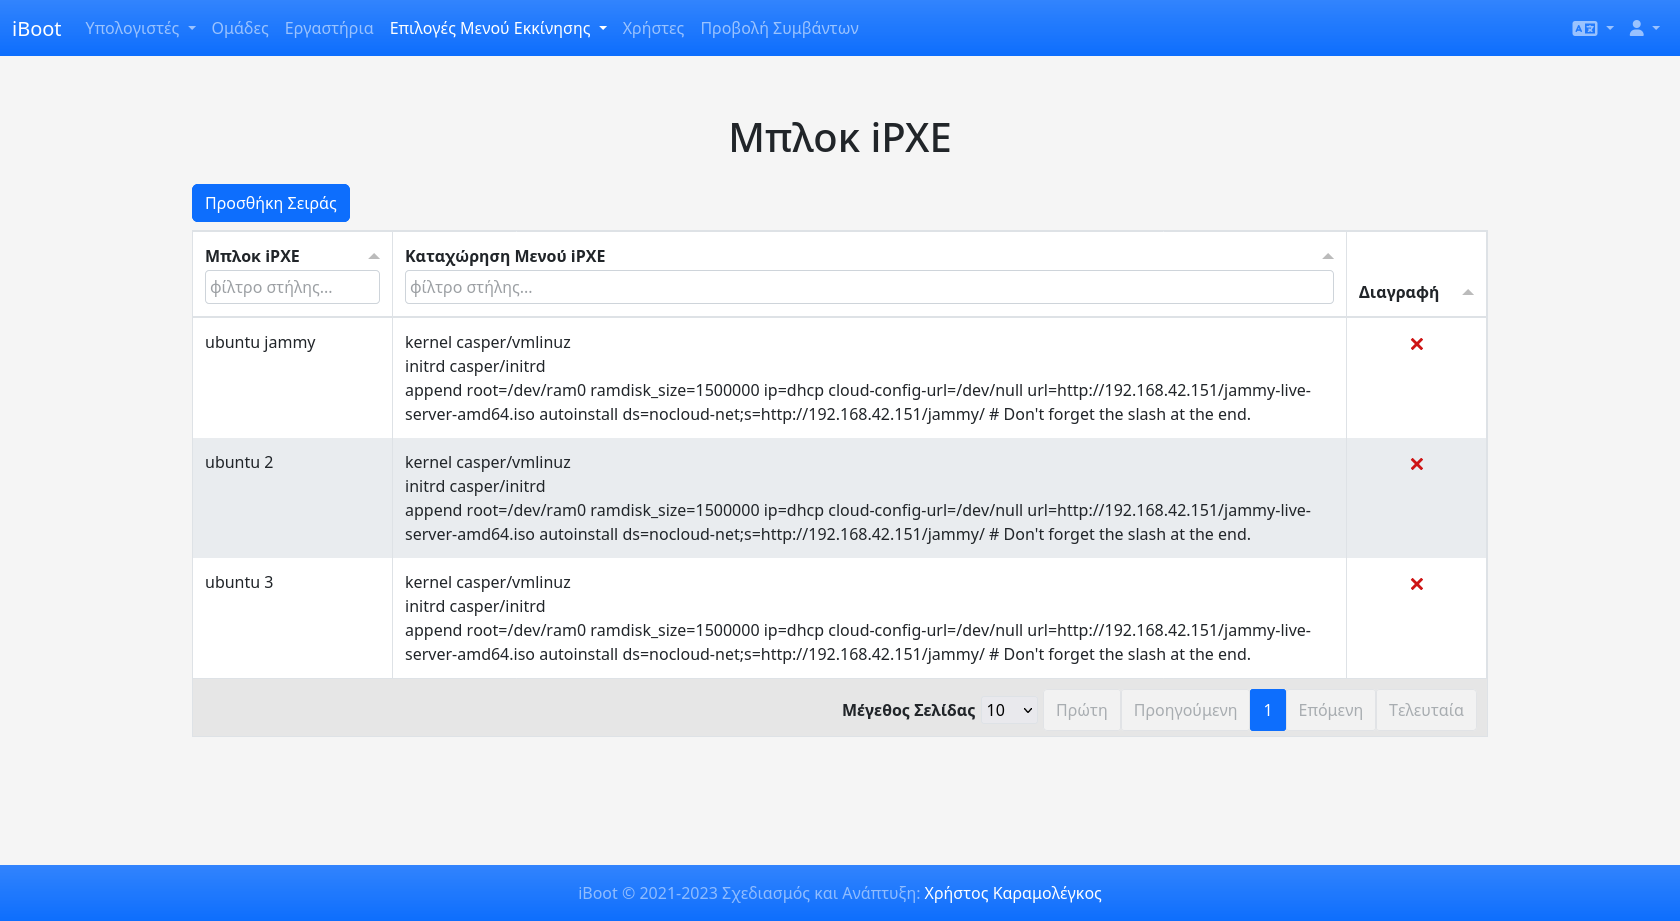
\includegraphics[scale=0.25]{iBoot-ipxeblocks.png}
	\caption{iBoot - Διαχείριση Μπλοκ Εντολών Τύπου iPXE}
	\label{fig:iBoot_ipxeblocks}
\end{figure}

H \emph{Καταχώρηση Μενού iPXE} είναι πεδίο ελεύθερου κειμένου, όπου ο χρήστης πρέπει να καταχωρήσει ένα έγκυρο μπλοκ iPXE. Μπορεί να χρησιμοποιήσει τις μεταβλητές \emph{\$\{group.ip\}} και \emph{\$\{group.prefix\}}, έτσι ώστε να γίνεται αυτόματη αντικατάστασή τους στο μενού που θα δημιουργείται, ανάλογα με το ποιο group περιείχε τον υπολογιστή που διαβάζει το μπλοκ.

Αν υπάρχει μπλοκ με όνομα \emph{default}, τότε σε περίπτωση που ζητήσει μενού κάποιος υπολογιστής που δεν έχει ενεργό πρόγραμμα εκκίνησης εκείνη τη στιγμή, θα λάβει ένα μενού με αυτό το μπλοκ.
\FloatBarrier

\subsection{Μενού Εκκίνησης}
\FloatBarrier
Στη σελίδα Μενού Εκκίνησης, προσβάσιμη στη διεύθυνση \verb!/boot_menu!, ο χρήστης μπορεί να προβάλει και να επεξεργαστεί τα μενού εκκίνησης που έχουν δημιουργηθεί, καθώς και να δημιουργήσει νέα.

Όπως φαίνεται στο σχήμα \ref{fig:iBoot_bootmenu}, ο πίνακας με τα στοιχεία των ομάδων αποτελείται από τις παρακάτω στήλες:
\begin{itemize}
	\item id: Το id του μενού εκκίνησης. Προβάλλεται για διευκόλυνση του διαχειριστή στη χειροκίνητη δοκιμή των μενού εκκίνησης
	\item Μενού Εκκίνησης: Το όνομα που έχει δοθεί στο μενού εκκίνησης
	\item Περιγραφή: Η περιγραφή του μενού εκκίνησης, για να μπορεί πιο εύκολα ο χρήστης να ξεχωρίσει τα μενού μεταξύ τους
	\item Μπλοκ iPXE: Ένα iPXE μπλοκ το οποίο αντιστοιχεί μόνο στο συγκεκριμένο μενού και εμφανίζεται κατά την εκκίνηση πριν από όλες τις άλλες εγγραφές που περιλαμβάνονται σε αυτό
	\item Επεξεργασία: Κουμπί για την επεξεργασία του μενού εκκίνησης, ως προς τα μπλοκ iPXE που περιέχει
	\item Διαγραφή: Κουμπί για τη διαγραφή του μενού εκκίνησης από το σύστημα
\end{itemize}

\begin{figure}[ht]
	\centering
	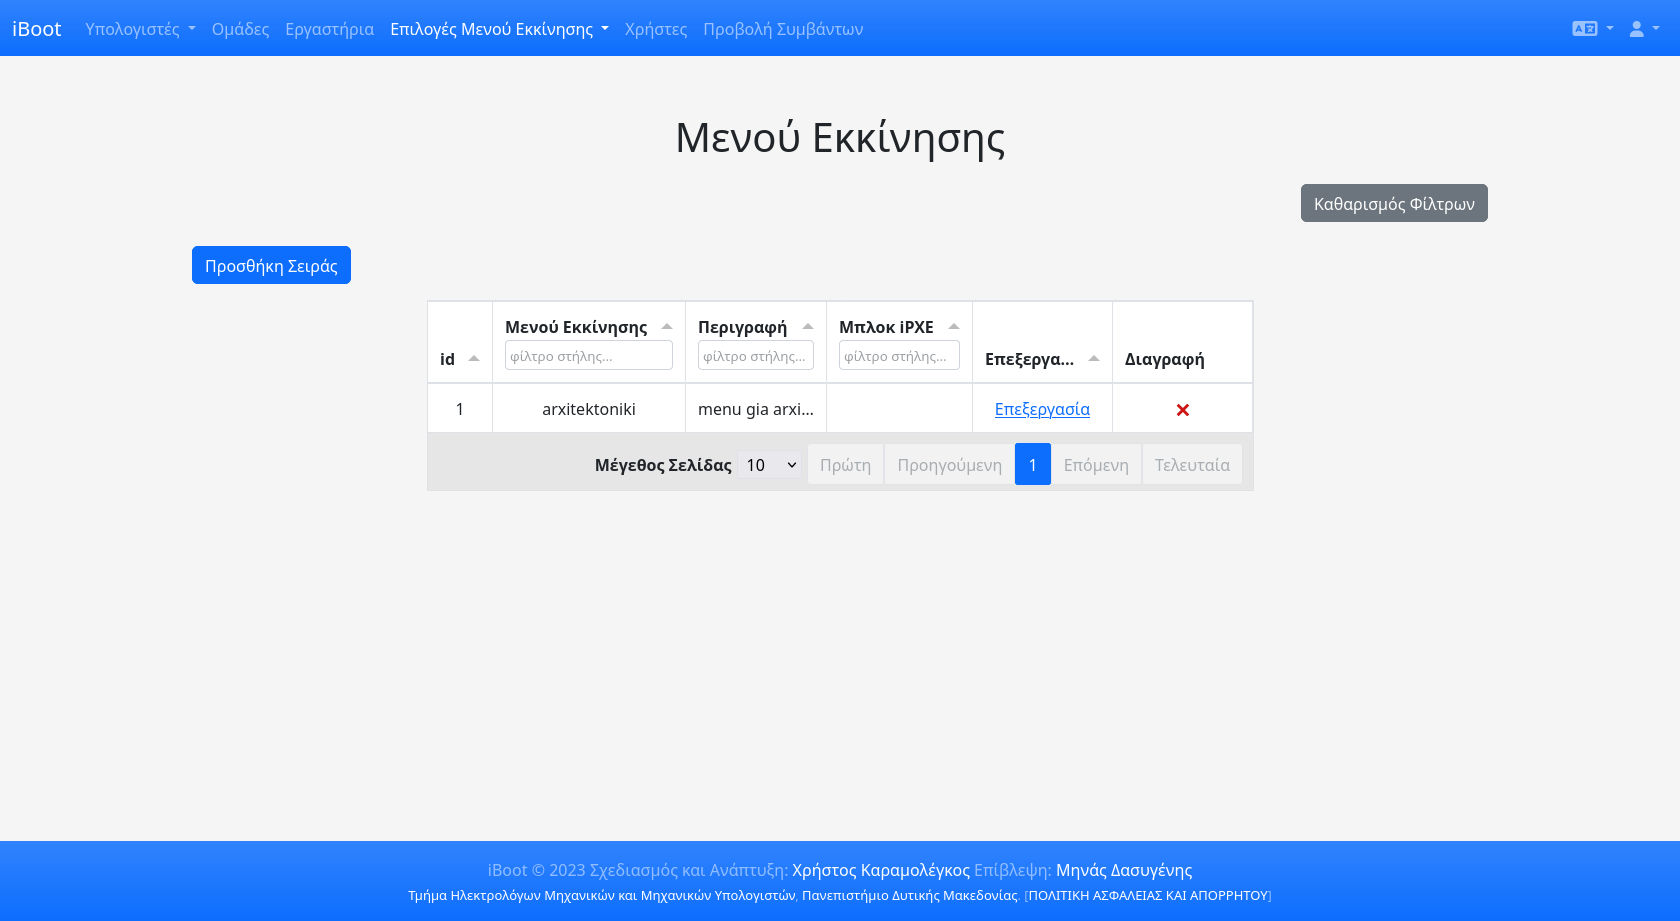
\includegraphics[scale=0.25]{iBoot-bootmenu.png}
	\caption{iBoot - Διαχείριση Μενού Εκκίνησης}
	\label{fig:iBoot_bootmenu}
\end{figure}

Πατώντας στην επεξεργασία ενός μενού, ο χρήστης μεταφέρεται στη σελίδα \verb!/boot_menu/{id}!, όπου μπορεί να προσθέσει ή να αφαιρέσει μπλοκ iPXE από τα υπάρχοντα στο συγκεκριμένο μενού εκκίνησης. Η σελίδα επεξεργασίας μενού απεικονίζεται στο σχήμα \ref{fig:iBoot_bootmenu_edit}.
\begin{figure}[ht]
	\centering
	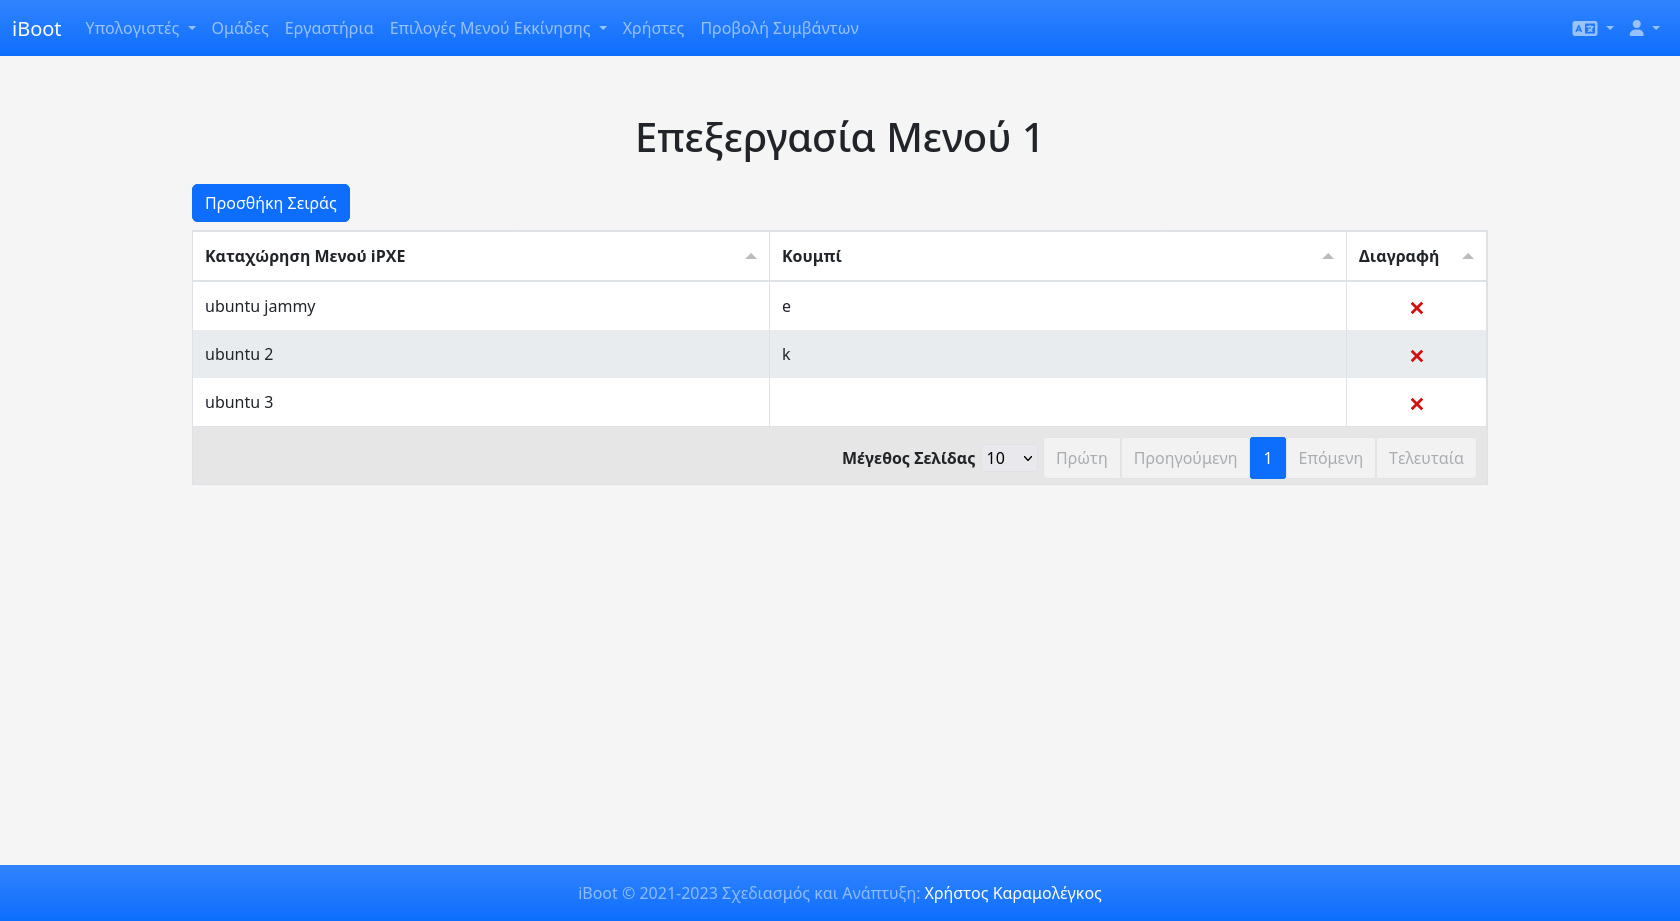
\includegraphics[scale=0.25]{iBoot-bootmenu_edit.png}
	\caption{iBoot - Επεξεργασία Μενού Εκκίνησης}
	\label{fig:iBoot_bootmenu_edit}
\end{figure}
\FloatBarrier

\subsection{Χρονοδιαγράμματα}
\FloatBarrier
Στη σελίδα Χρονοδιαγράμματα, προσβάσιμη στη διεύθυνση \verb!/schedules!, ο χρήστης μπορεί να προβάλει και να επεξεργαστεί τα χρονοδιαγράμματα που έχουν δημιουργηθεί, καθώς και να δημιουργήσει νέα. Τα υπάρχοντα ενεργά χρονοδιαγράμματα απεικονίζονται σε ένα ημερολόγιο, ώστε να είναι ευκολότερος ο προσδιορισμός τους από τον χρήστη, και η κατανόηση του μενού που θα δημιουργηθεί για μια ομάδα σε κάποια συγκεκριμένη χρονική στιγμή.

Όπως φαίνεται στο σχήμα \ref{fig:iBoot_schedules}, ο πίνακας με τα στοιχεία των χρονοδιαγραμμάτων αποτελείται από τις παρακάτω στήλες:
\begin{itemize}
	\item Ώρα Από: Η ώρα από την οποία θα είναι ενεργό το χρονοδιάγραμμα
	\item Ώρα Έως: Η ώρα έως την οποία θα είναι ενεργό το χρονοδιάγραμμα
	\item Ημέρα Εβδομάδας: Η ημέρα της εβδομάδας για την οποία θα είναι ενεργό το χρονοδιάγραμμα
	\item Ημερομηνία: Η συγκεκριμένη ημερομηνία για την οποία θα είναι ενεργό το χρονοδιάγραμμα
	\item Μενού Εκκίνησης: Το μενού εκκίνησης που θα δοθεί στα μηχανήματα που θα ζητήσουν να εκκινηθούν εντός χρονικών πλαισίων του χρονοδιαγράμματος
	\item Ομάδα: Η ομάδα της οποίας οι υπολογιστές-μέλη μπορούν να αιτηθούν μενού εκκίνησης από το συγκεκριμένο χρονοδιάγραμμα
	\item Ενεργό: Πεδίο με πλαίσιο επιλογής που καθορίζει αν είναι ενεργό ή όχι το χρονοδιάγραμμα
	\item Δημιουργήθηκε στις: Πεδίο μόνο για ανάγνωση, περιέχει την χρονοσφραγίδα δημιουργίας του χρονοδιαγράμματος
	\item Ενημερώθηκε στις: Πεδίο μόνο για ανάγνωση, περιέχει την χρονοσφραγίδα τελευταίας ενημέρωσης του χρονοδιαγράμματος
	\item Διαγραφή: Κουμπί για τη διαγραφή του χρονοδιαγράμματος από το σύστημα
\end{itemize}

\begin{figure}[ht]
	\centering
	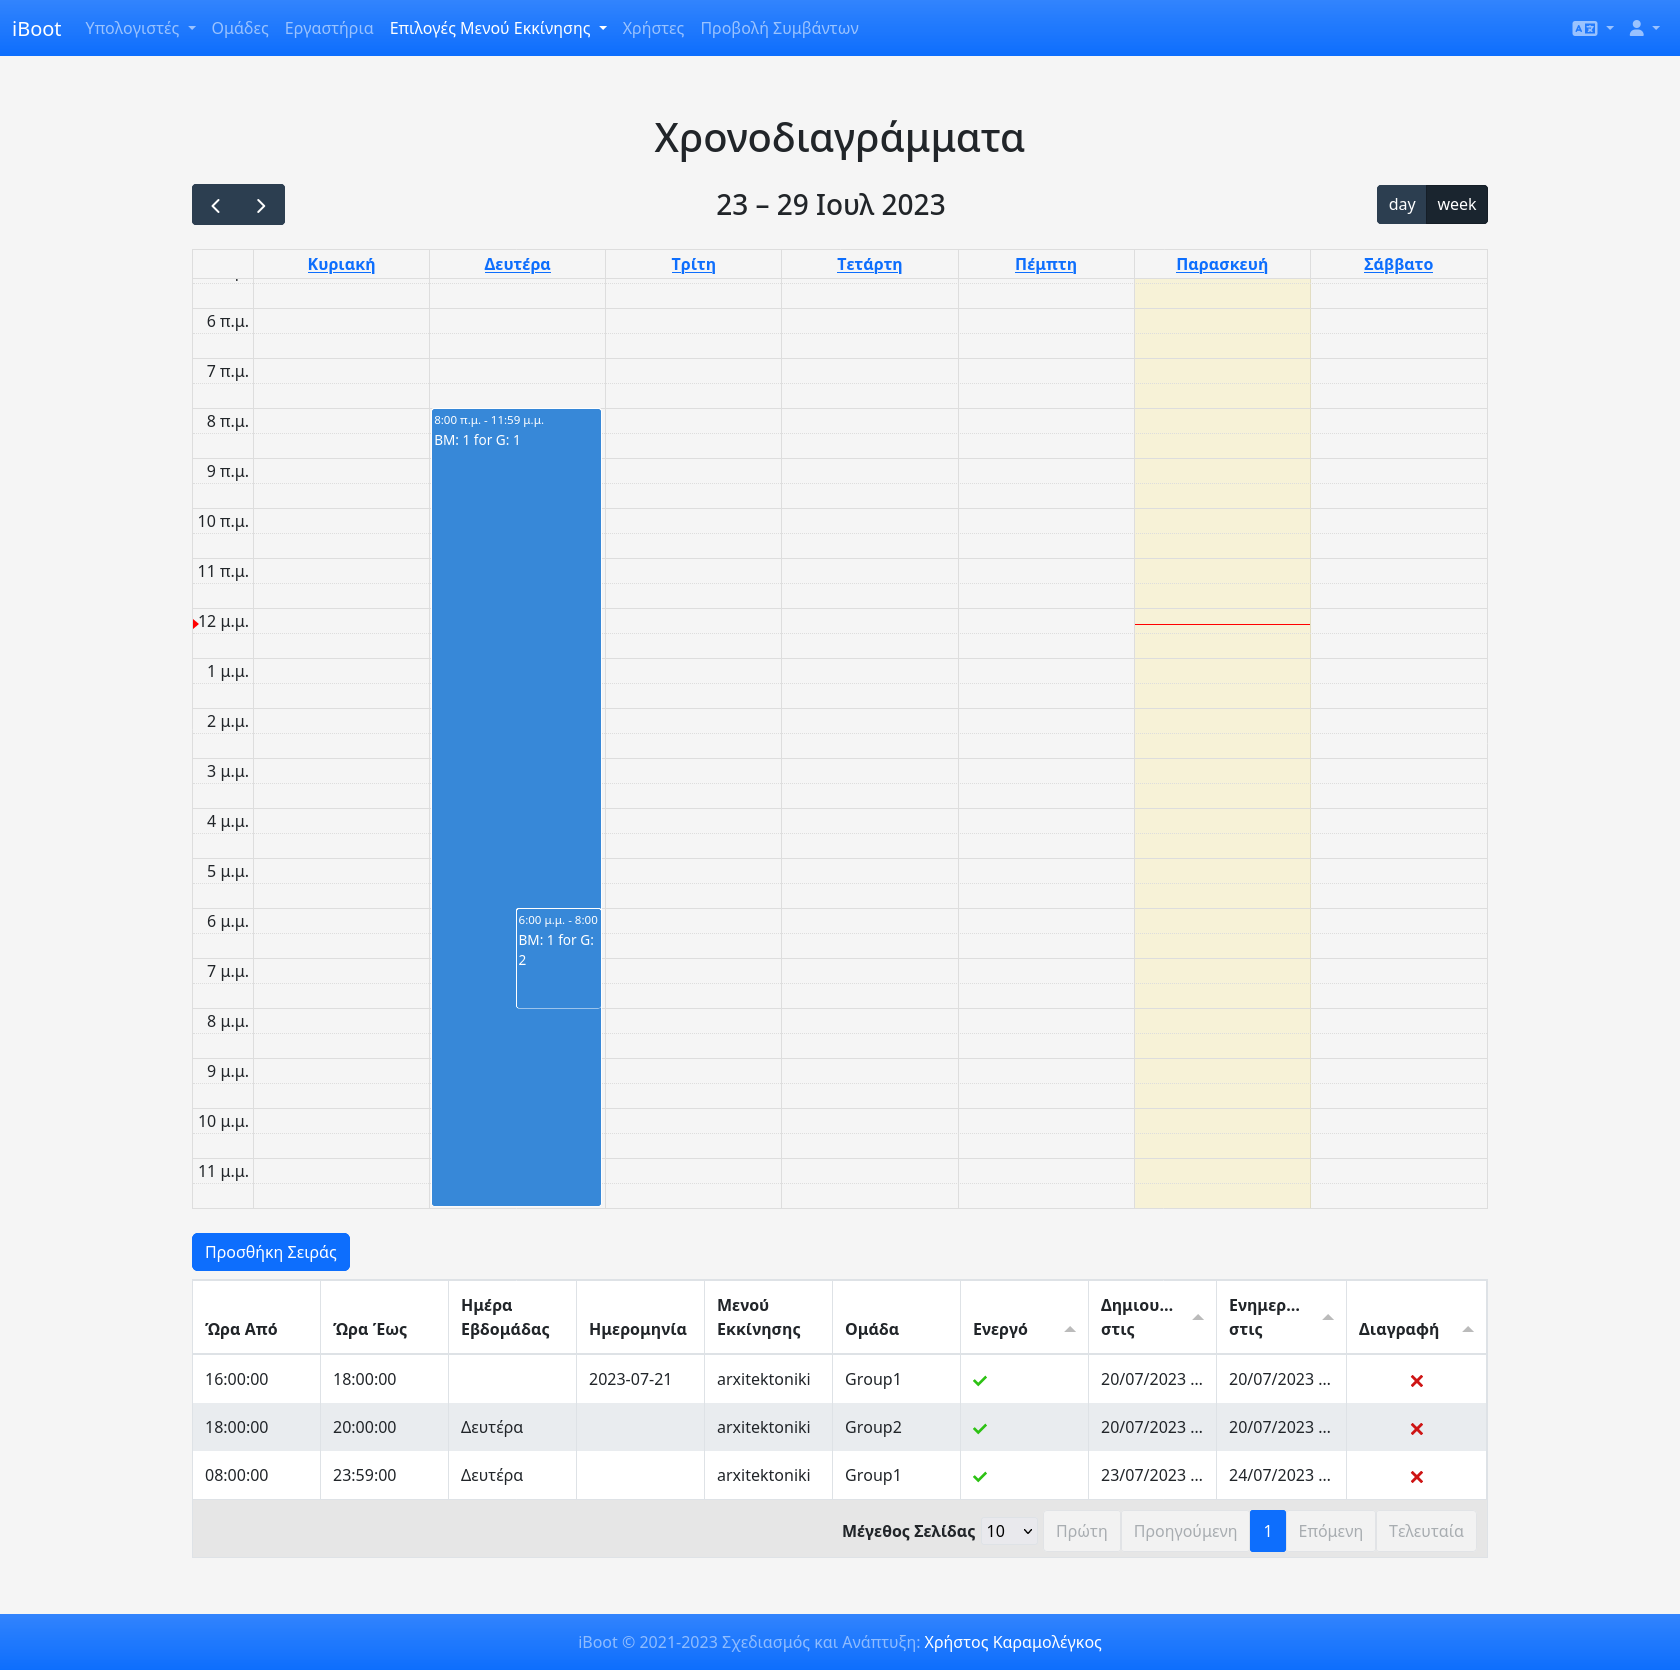
\includegraphics[scale=0.25]{iBoot-schedules.png}
	\caption{iBoot - Διαχείριση Χρονοδιαγραμμάτων}
	\label{fig:iBoot_schedules}
\end{figure}
Για τη δημιουργία χρονοδιαγράμματος, είναι απαραίτητο μόνο ένα από τα πεδία \emph{Ημέρα Εβδομάδας} και \emph{Ημερομηνία}. Αν έχει οριστεί το πεδίο \emph{Ημέρα Εβδομάδας}, τότε το χρονοδιαγραμμα θα είναι επαναλαμβανόμενο και θα ενεργοποιείται κάθε εβδομάδα, την ημέρα που είναι δηλωμένη στο πεδίο. Αν έχει οριστεί το πεδίο \emph{Ημερομηνία}, τότε το χρονοδιαγραμμα δεν θα είναι επαναλαμβανόμενο και θα ενεργοποιηθεί μόνο τη συγκεκριμένη ημερομηνία που είναι δηλωμένη στο πεδίο. Αν τύχει για μια χρονική στιγμή να είναι ταυτόχρονα ενεργά για την ίδια ομάδα υπολογιστών δύο χρονοδιαγράμματα, εκ των οποίων το ένα έχει ορισμένο το πεδίο \emph{Ημέρα Εβδομάδας} και το άλλο το πεδίο \emph{Ημερομηνία}, τότε το χρονοδιάγραμμα με τη συγκεκριμένη ημερομηνία έχει προτεραιότητα και υπερκαλύπτει το άλλο.
\FloatBarrier

\subsection{Χρήστες}
\FloatBarrier
Στη σελίδα Χρήστες, προσβάσιμη μόνο από διαχειριστές στη διεύθυνση \verb!/users!, ο χρήστης μπορεί να προβάλει και να επεξεργαστεί τα στοιχεία των χρηστών της εφαρμογής.

Όπως φαίνεται στο σχήμα \ref{fig:iBoot_users}, ο πίνακας με τα στοιχεία των χρηστών αποτελείται από τις παρακάτω στήλες:
\begin{itemize}
	\item Ονοματεπώνυμο: Το ονοματεπώνυμο του χρήστη
	\item Email: Η διεύθυνση email του χρήστη
	\item Τηλέφωνο: Ο αριθμός τηλεφώνου του χρήστη
	\item Όνομα Χρήστη: Το όνομα χρήστη (username) που χρησιμοποιείται για ταυτοποίηση στο σύστημα
	\item Κωδικός: Ο κωδικός πρόσβασης του χρήστη
	\item Διαχειριστής: Πεδίο με πλαίσιο επιλογής που καθορίζει αν είναι διαχειριστής ή όχι ο χρήστης
	\item Επιβεβαιωμένο Email: Πεδίο με πλαίσιο επιλογής που καθορίζει αν είναι είναι επιβεβαιωμένο ή όχι το email του χρήστη
	\item Εργαστήρια: Λίστα των εργαστηρίων που έχουν ανατεθεί στον χρήστη, αν αυτός δεν είναι διαχειριστής
	\item Δημιουργήθηκε στις: Πεδίο μόνο για ανάγνωση, περιέχει την χρονοσφραγίδα δημιουργίας του χρονοδιαγράμματος
	\item Ενημερώθηκε στις: Πεδίο μόνο για ανάγνωση, περιέχει την χρονοσφραγίδα τελευταίας ενημέρωσης του χρονοδιαγράμματος
	\item Διαγραφή: Κουμπί για τη διαγραφή του χρήστη από το σύστημα
\end{itemize}

\begin{figure}[ht]
	\centering
	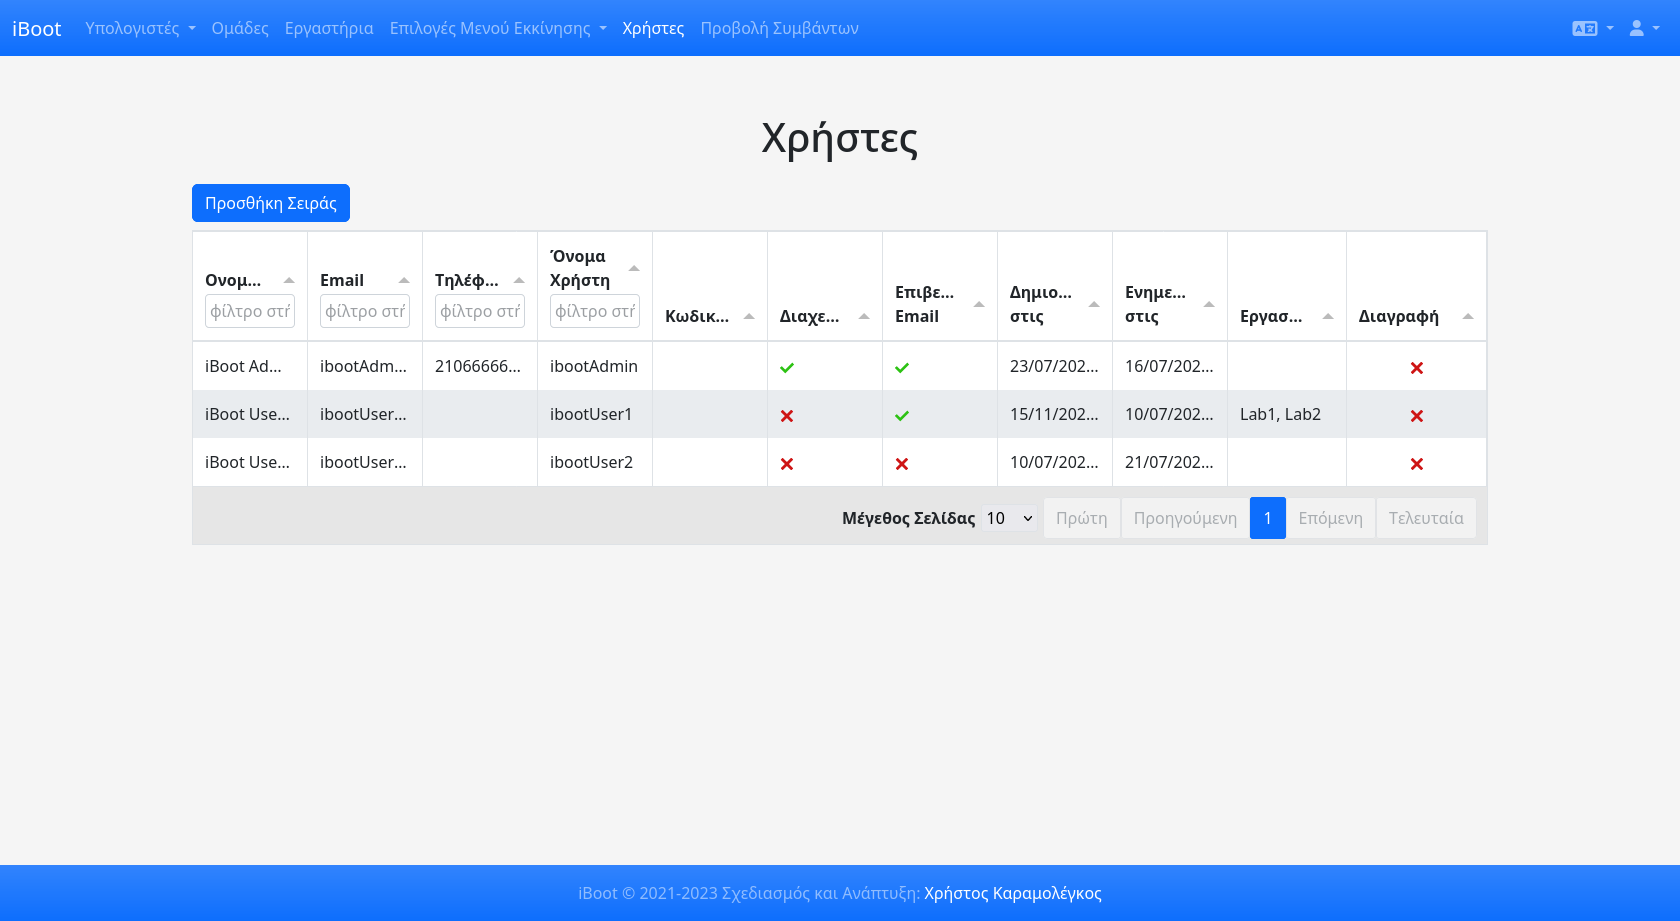
\includegraphics[scale=0.25]{iBoot-users.png}
	\caption{iBoot - Διαχείριση Χρηστών}
	\label{fig:iBoot_users}
\end{figure}
Το πεδίο \emph{Κωδικός} φαίνεται κενό, καθώς οι κωδικοί αποθηκεύονται κρυπτογραφημένοι στη βάση δεδομένων της εφαρμογής και οι κρυπτογραφημένες συμβολοσειρές δεν εμφανίζονται σε κανένα σημείο της εφαρμογής. Το πεδίο είναι εγγράψιμο και υπάρχει για την αλλαγή του κωδικού του κάθε χρήστη.
\FloatBarrier

\subsection{Συμβάντα}
\FloatBarrier
Στη σελίδα των Συμβάντων, προσβάσιμη μόνο από διαχειριστές στη διεύθυνση \verb!/logs!, ο χρήστης μπορεί να δει τις καταγραφές συμβάντων που έχουν δημιουργηθεί από την εφαρμογή.

Όπως φαίνεται στο σχήμα \ref{fig:iBoot_logs}, ο πίνακας με τα στοιχεία των Μπλοκ iPXE αποτελείται από τις παρακάτω στήλες:
\begin{itemize}
	\item Επίπεδο: Το όνομα που έχει δοθεί στο Μπλοκ iPXE
	\item Ημερομηνία: Το περιεχόμενο της καταχώρησης μπλοκ iPXE
	\item Περιεχόμενο: Κουμπί για τη διαγραφή του Μπλοκ iPXE από το σύστημα
\end{itemize}

\begin{figure}[ht]
	\centering
	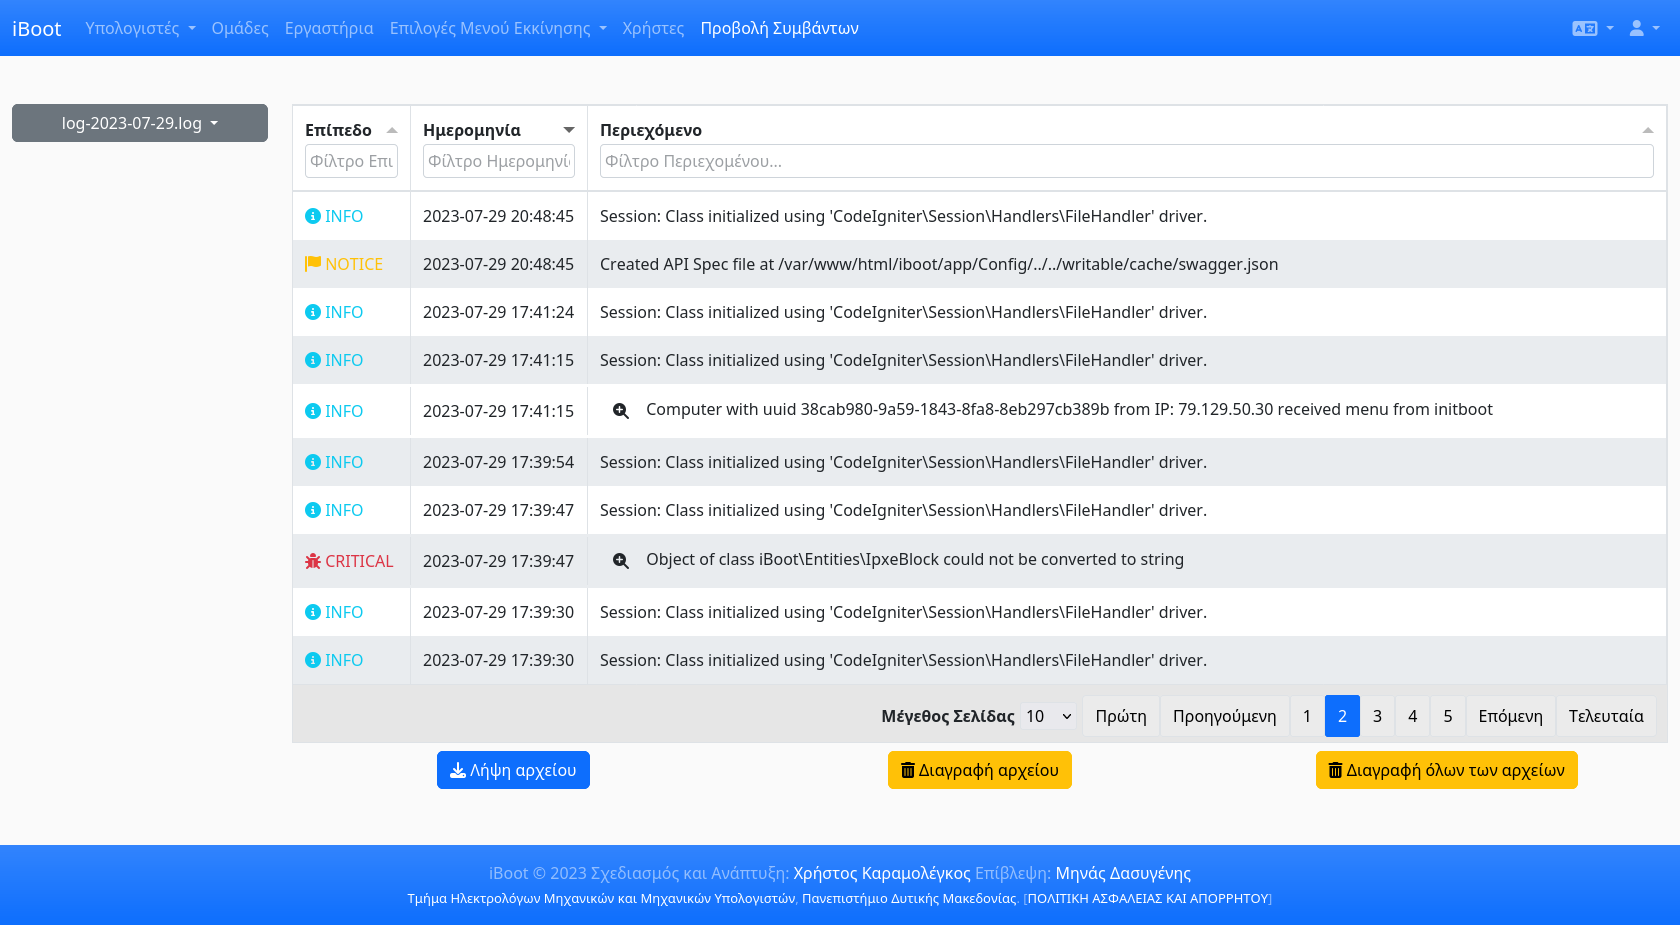
\includegraphics[scale=0.25]{iBoot-logs.png}
	\caption{iBoot - Συμβάντα}
	\label{fig:iBoot_logs}
\end{figure}
Στο αριστερό μέρος της σελίδας, υπάρχει ένας επιλογέας του αρχείου καταγραφής συμβάντων που θέλει να προβάλει ο χρήστης, με προεπιλεγμένο αυτό της τρέχουσας ημερομηνίας. Επιλέγοντας ένα αρχείο, αν είναι πολύ μεγάλο για προβολή ο χρήστης προτρέπεται να το μεταφορτώσει για να το προβάλει τοπικά στη συσκευή του, διαφορετικά οι εγγραφές του αρχείου γεμίζουν τον πίνακα.

Ο χρήστης έχει τη δυνατότητα να επιλέξει αν θα εμφανίζονται στον πίνακα 10, 25, 50 ή 100 εγγραφές, ενώ αν υπάρχουν περισσότερες σελιδοποιούνται αυτόματα. Επίσης, μπορεί να φιλτράρει τις εγγραφές ανάλογα με το επίπεδό τους, την ημερομηνία ή το περιεχόμενό τους, κάνοντας έτσι εύκολη την αναζήτηση συγκεκριμένων εγγραφών.

Τέλος, δίνεται η δυνατότητα να γίνει λήψη ή διαγραφή του αρχείου που προβάλει ο χρήστης, καθώς και διαγραφή όλων των αρχείων καταγραφής συμβάντων.
\FloatBarrier

\subsection{Ρύθμιση Εκκίνησης Υπολογιστών}
\FloatBarrier
Στη σελίδα των Ρύθμισης Εκκίνησης Υπολογιστών, προσβάσιμη στη διεύθυνση \verb!/boot!, δίνονται οδηγίες παραμετροποίησης του DHCP Server από τον οποίο θα ζητήσουν διαδικτυακή εκκίνηση οι υπολογιστές όταν εκκινηθούν. Συγκεκριμένα, υπάρχουν οδηγίες ρύθμισης για ICS DHCPD και Dnsmasq, ενώ ο χρήστης παροτρύνεται να αναζητήσει οδηγίες ρύθμισης στις οδηγίες χρήστη του DHCP Server του, αν χρησιμοποιεί κάποιον διαφορετικό.
Η σελίδα Ρύθμισης Εκκίνησης Υπολογιστών απεικονίζεται στο σχήμα \ref{fig:iBoot_boot}.
\begin{figure}[ht]
	\centering
	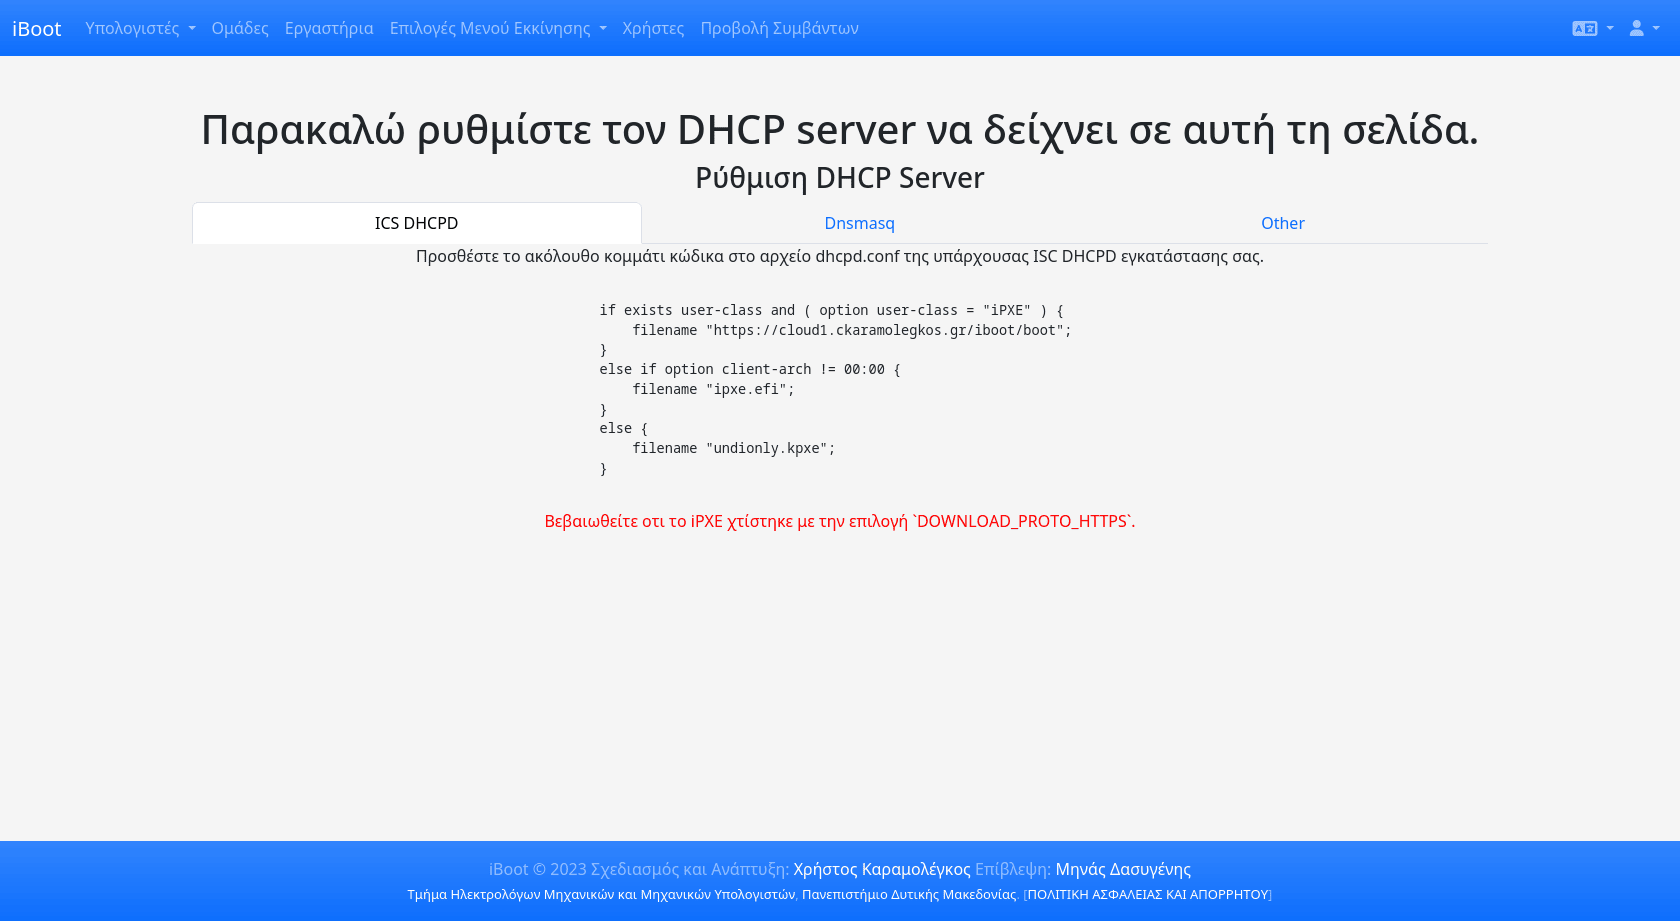
\includegraphics[scale=0.25]{iBoot-boot.png}
	\caption{iBoot - Ρύθμιση Εκκίνησης Υπολογιστών}
	\label{fig:iBoot_boot}
\end{figure}
\FloatBarrier

\subsection{Προδιαγραφή API}
\FloatBarrier
Η σελίδα της Προδιαγραφής API, προσβάσιμη στη διεύθυνση \verb!/api!, περιέχει μια λεπτομερή καταγραφή των REST API endpoints της εφαρμογής. Οι εγγραφές είναι λειτουργικές, αφού ο χρήστης μπορεί να πραγματοποιήσει αιτήματα στο API της εφαρμογής μέσω της σελίδας, πατώντας το κουμπί "Try it out" της εγγραφής που θέλει να δοκιμάσει. Εκτελώντας ένα αίτημα σε κάποιο endpoint του API, εμφανίζεται και η αντίστοιχη curl εντολή που θα μπορούσε να εκτελέσει ο χρήστης για να πραγματοποιήσει το ίδιο αίτημα.

Φυσικά, όλα τα endpoints είναι κλειδωμένα και απαιτούν τη χρήση JWT token για να αυθεντικοποιηθεί ο χρήστης που εκτελεί το κάθε αίτημα και να διαπιστωθεί ότι έχει τα απαραίτητα δικαιώματα. Το endpoint της σύνδεσης χρήστη \verb!/api/user/login! είναι ανοιχτό για POST αιτήματα, ώστε ο χρήστης να μπορεί με χρήση του ονόματος χρήστη και του κωδικού πρόσβασής του, να λάβει το JWT token το οποίο πρέπει να επισυνάπτει σε όλα τα επόμενα αιτήματα προς τα κλειδωμένα endpoints, για την εξυπηρέτησή τους. Πατώντας το κουμπί "Authorize" στο πάνω μέρος της σελίδας, ο χρήστης μπορεί να προσθέσει στο πλαίσιο που εμφανίζεται το JWT token του, ώστε να επισυνάπτεται αυτόματα σε όλα τα επόμενα αιτήματα που θα πραγματοποιήσει. Αν ο χρήστης έχει συνδεθεί στην εφαρμογή ήδη, όταν επισκεφτεί τη σελίδα Προδιαγραφής API, το token του επισυνάπτεται αυτόματα.

Η σελίδα της Προδιαγραφής API απεικονίζεται στο σχήμα \ref{fig:iBoot_api_spec}.
\begin{figure}[ht]
	\centering
	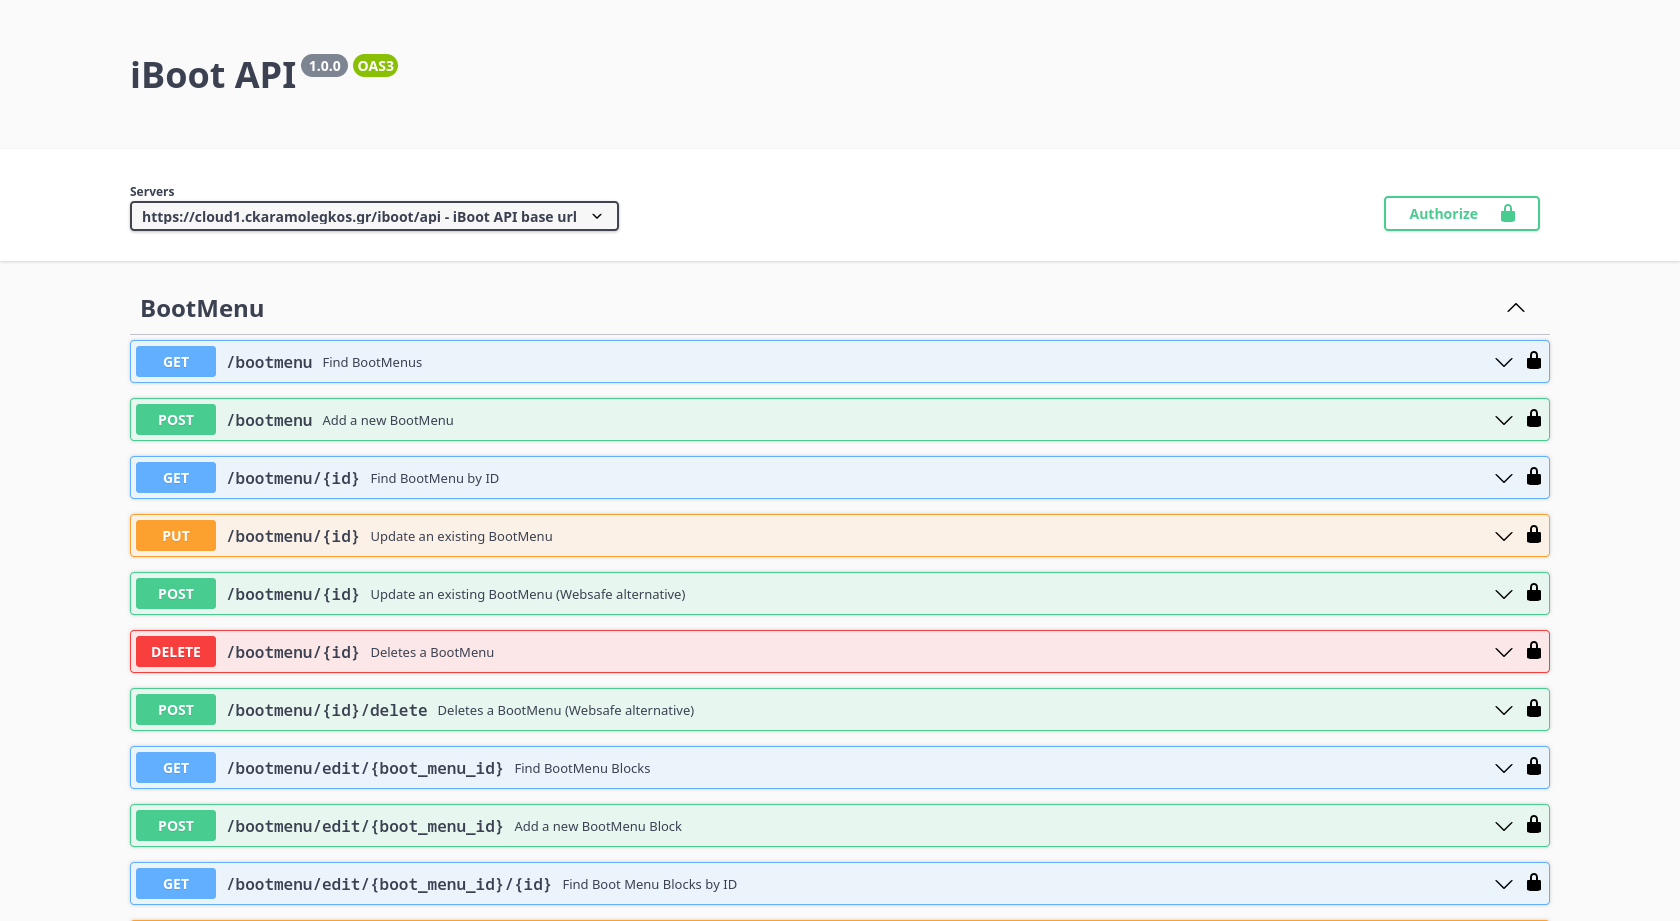
\includegraphics[scale=0.25]{iBoot-api_spec.png}
	\caption{iBoot - Προδιαγραφή API}
	\label{fig:iBoot_api_spec}
\end{figure}
\FloatBarrier

\section{Επεξήγηση Αρχείων}
Καθώς η διαδικτυακή εφαρμογή αναπτύχθηκε με χρήση του CodeIgniter 4 Framework, χρησιμοποιεί και τη δομή αρχείων του \cite{CodeIgniter_structure}.

\subsection{Βασική Δομή CodeIgniter 4}
Η βασική δομή της εφαρμογής αποτελείται από πέντε καταλόγους: \hyperref[ui:app]{app/}, \hyperref[ui:public]{public/}, \hyperref[ui:writable]{writable/}, \hyperref[ui:tests]{tests/} και \hyperref[ui:system]{vendor/ ή system/}.

\subsubsection{app} \label{ui:app}
Στον κατάλογο app βρίσκεται όλος ο κώδικας της εφαρμογής. Οι ακόλουθοι φάκελοι αποτελούν τα βασικά περιεχόμενα:\\

\begin{figure} 
	\centering 
	{\footnotesize
	\begin{forest}
		pic dir tree,
		pic root,
		for tree={% folder icons by default; override using file for file icons
			directory,
			fit=band
		},
		[app/
			[Config/ \ \ \ \ \ \ Αρχεία ρύθμισης παραμέτρων της εφαρμογής]
			[Controllers/ \ Οι Controllers που καθορίζουν τη ροή του προγράμματος]
			[Database/ \ \ \ \ Κλάσεις για την ενημέρωση του σχήματος και την αρχικοποίηση βάσεων δεδομένων]
			[Filters/ \ \ \ \ \ Κλάσεις φίλτρων που μπορούν να εκτελούνται πριν και μετά τους controllers]
			[Helpers/ \ \ \ \ \ Συλλογές αυτόνομων βοηθητικών συναρτήσεων]
			[Language/ \ \ \ \ Συμβολοσειρές γλώσσας για την υποστήριξη πολλαπλών γλωσσών]
			[Libraries/ \ \ \ Χρήσιμες κλάσεις που δεν ταιριάζουν σε άλλη κατηγορία]
			[Models/ \ \ \ \ \ \ Τα Models που διασυνδέουν την εφαρμογή με τη βάση δεδομένων]
			[ThirdParty/ \ \ Βιβλιοθήκες τρίτων που μπορούν να χρησιμοποιηθούν στην εφαρμογή]
			[Views/ \ \ \ \ \ \ \ Τα Views που συνθέτουν την HTML που εμφανίζεται στον πελάτη]
		]
	\end{forest}
	}
	\caption{Η βασική δομή του CodeIgniter 4 framework}
	\label{dir:ci4}
\end{figure}

Στον κατάλογο app έχει δοθεί το php namespace `iBoot', έτσι ώστε τα ονόματα των αρχείων που βρίσκονται στους υποκαταλόγους του να μην συγκρούονται με ομοίως ονομαζόμενα αρχεία του Framework ή άλλων χρησιμοποιούμενων βιβλιοθηκών.

\subsubsection{public} \label{ui:public}
Ο κατάλογος public περιέχει το προσβάσιμο από το πρόγραμμα περιήγησης τμήμα της διαδικτυακής εφαρμογής, αποτρέποντας την άμεση πρόσβαση στον πηγαίο κώδικα. Περιέχει το κύριο αρχείο .htaccess, το index.php και όλα τα επιπρόσθετα στοιχεία της εφαρμογής, όπως CSS, javascript και εικόνες.

Αυτός ο φάκελος προορίζεται να είναι η "διαδικτυακή ρίζα" της εφαρμογής και ο διακομιστής ιστού θα πρέπει να ρυθμιστεί ώστε να δείχνει σε αυτόν.

\subsubsection{writable} \label{ui:writable}
Αυτός ο κατάλογος περιέχει όλους τους καταλόγους στους οποίους μπορεί να χρειαστεί να γίνει εγγραφή αρχείων κατά τη διάρκεια της ζωής της εφαρμογής. Αυτό περιλαμβάνει καταλόγους για την αποθήκευση προσωρινών αρχείων cache, αρχείων καταγραφής συμβάντων και τυχόν μεταφορτώσεις που μπορεί να στείλει ένας χρήστης. Θα πρέπει να προστεθούν εκεί όλοι οι κατάλογοι στους οποίους θα χρειαστεί να γράψει η εφαρμογή. Αυτό επιτρέπει τον ορισμό των υπόλοιπων κύριων καταλόγων ως μη εγγράψιμους, ως πρόσθετο μέτρο ασφαλείας κατά της ανεπιθύμητης τροποποίησης του κώδικα της εφαρμογής.

\subsubsection{tests} \label{ui:tests}
Αυτός ο κατάλογος έχει οριστεί για να περιέχει τα αρχεία δοκιμών. Ο κατάλογος \_support περιέχει διάφορες κλάσεις προσομοίωσης και άλλα βοηθητικά προγράμματα που μπορούν να χρησιμοποιηθούν για τη συγγραφή και εκτέλεση δοκιμών. Αυτός ο κατάλογος δεν χρειάζεται να υπάρχει στην παραγωγική εγκατάσταση της εφαρμογής.

\subsubsection{system} \label{ui:system}
Αυτός ο κατάλογος περιέχει τα αρχεία που συνθέτουν το ίδιο το CodeIgniter 4 Framework. Tα αρχεία στον κατάλογο συστήματος δεν πρέπει ποτέ να τροποποιούνται. Αντ' αυτού, μπορούν να επεκταθούν οι υπάρχουσες κλάσεις ή να δημιουργήθούν νέες, ώστε να παρέχουν την επιθυμητή λειτουργικότητα.

Όλα τα αρχεία σε αυτόν τον κατάλογο βρίσκονται κάτω από το php namespace `CodeIgniter'.

Η εγκατάσταση του framework έχει γίνει με τη βοήθεια του Composer, οπότε στην περίπτωσή μας, ο κατάλογος συστήματος βρίσκεται στη διαδρομή `vendor/codeigniter4/framework/system'.

\FloatBarrier
\subsection{Δομή Αρχείων iBoot}
Τα αρχεία που έχουν δημιουργηθεί για τη λειτουργία της εφαρμογής και του REST API της, τον καθορισμό της εμφάνισής της, αλλά και της επικοινωνίας της με τη βάση δεδομένων της, περιέχονται στον φάκελο \emph{app} και περιγράφονται αναλυτικά παρακάτω.

\subsubsection{Controllers} \label{ui:app:controllers}
Στον κατάλογο Controllers βρίσκονται οι ελεγκτές που είναι υπεύθυνοι για την επιχειρησιακή λογική της εφαρμογής. Τα περιεχόμενα του καταλόγου Controllers απεικονίζονται στο σχήμα \ref{dir:iBoot-Controllers}.

\begin{figure}
	\centering
	{\footnotesize
	\begin{forest}
		pic dir tree,
		pic root,
		for tree={% folder icons by default; override using file for file icons
			directory,
			fit=band
		},
		[Controllers/ \ \ \ \ \ \ \ \ \ \ \ \ Αρχεία ελεγκτών υπεύθυνων για την επιχειρησιακή λογική της εφαρμογής
			[Api/ \ \ \ \ \ \ \ \ \ \ \ \ \ \ \ \ \ \ Ελεγκτές του REST API της εφαρμογής
				[ApiLogViewer.php \ \ \ Η συνάρτηση προβολής και διαγραφής των αρχείων καταγραφής συμβάντων, file]
				[BootMenu.php \ \ \ \ \ \ \ Οι CRUD συναρτήσεις των Μενού Εκκίνησης, file]
				[BootMenuBlocks.php \ Οι CRUD συναρτήσεις των Μπλοκ iPXE των Μενού Εκκίνησης, file]
				[Computer.php \ \ \ \ \ \ \ Οι CRUD συναρτήσεις των Υπολογιστών, file]
				[Group.php \ \ \ \ \ \ \ \ \ \ Οι CRUD συναρτήσεις των Ομάδων, file]
				[IpxeBlock.php \ \ \ \ \ \ Οι CRUD συναρτήσεις των Μπλοκ iPXE, file]
				[Lab.php \ \ \ \ \ \ \ \ \ \ \ \ Οι CRUD συναρτήσεις των Εργαστηρίων, file]
				[Schedule.php \ \ \ \ \ \ \ Οι CRUD συναρτήσεις των Χρονοδιαγραμμάτων, file]
				[Swagger.php \ \ \ \ \ \ \ \ Ο ελεγκτής απεικόνισης της προδιαγραφής του REST API, file]
				[User.php \ \ \ \ \ \ \ \ \ \ \ Οι CRUD συναρτήσεις των Χρηστών, file]
			]
			[BaseController.php \ \ \ \ Ο βασικός ελεγκτής τον οποίο επεκτείνουν οι υπόλοιποι, file]
			[BootMenu.php \ \ \ \ \ \ \ \ \ \ Ο ελεγκτής προβολής των Μενού Εκκίνησης, file]
			[Computers.php \ \ \ \ \ \ \ \ \ Ο ελεγκτής προβολής των Υπολογιστών, file]
			[Dashboard.php \ \ \ \ \ \ \ \ \ Ο ελεγκτής προβολής της αρχικής σελίδας, file]
			[Groups.php \ \ \ \ \ \ \ \ \ \ \ \ Ο ελεγκτής προβολής των Ομάδων, file]
			[Home.php \ \ \ \ \ \ \ \ \ \ \ \ \ \ Ο ελεγκτής αρχικής ανακατεύθυνσης και προβολής των σελίδων εκκίνησης, file]
			[IpxeBlocks.php \ \ \ \ \ \ \ \ Ο ελεγκτής προβολής των Μπλοκ iPXE, file]
			[Labs.php \ \ \ \ \ \ \ \ \ \ \ \ \ \ Ο ελεγκτής προβολής των Εργαστηρίων, file]
			[Locale.php \ \ \ \ \ \ \ \ \ \ \ \ Ο ελεγκτής αλλαγής γλώσσας, file]
			[LogViewer.php \ \ \ \ \ \ \ \ \ Ο ελεγκτής προβολής των αρχείων καταγραφής συμβάντων, file]
			[Schedules.php \ \ \ \ \ \ \ \ \ Ο ελεγκτής προβολής των Χρονοδιαγραμμάτων, file]
			[User.php \ \ \ \ \ \ \ \ \ \ \ \ \ \ Ο ελεγκτής προβολής των Χρηστών, file]
		]
	\end{forest}
	}
	\caption{Τα αρχεία του καταλόγου Controllers του iBoot}
	\label{dir:iBoot-Controllers}
\end{figure}

\subsubsection{Database} \label{ui:app:database}
Στον κατάλογο Database βρίσκονται τα αρχεία υπεύθυνα για τον καθορισμό του σχήματος της βάσης δεδομένων και της αρχικοποίησης δεδομένων, αν αυτό χρειάζεται. Τα περιεχόμενα του καταλόγου Database απεικονίζονται στο σχήμα \ref{dir:iBoot-Database}.

\begin{figure}
	\centering
	{\footnotesize
		\begin{forest}
			pic dir tree,
			pic root,
			for tree={% folder icons by default; override using file for file icons
				directory,
				fit=band
			},
			[Database/ \ \ \ \ \ \ \ \ \ \ \ \ \ \ \ \ \ \ \ \ \ \ \ \ \ Κλάσεις σχεδιασμού και αρχικοποίησης της βάσης δεδομένων
				[Migrations/ \ \ \ \ \ \ \ \ \ \ \ \ \ \ \ \ \ \ \ \ \ Κλάσεις ενημέρωσης του σχήματος της βάσης δεδομένων
					[2022-06-27-172100\_InitDB.php \ Κατασκευάζει το σχήμα της βάσης δεδομένων, file]
				]
				[Seeds/ \ \ \ \ \ \ \ \ \ \ \ \ \ \ \ \ \ \ \ \ \ \ \ \ \ \ Κλάσεις αρχικοποίησης τη βάση δεδομένων με εγγραφές]
			]
		\end{forest}
	}
	\caption{Τα αρχεία του καταλόγου Database του iBoot}
	\label{dir:iBoot-Database}
\end{figure}

\subsubsection{Entities} \label{ui:app:entities}
Στον κατάλογο Entities βρίσκονται οι κλάσεις οντοτήτων της εφαρμογής. Οι οντότητες λειτουργούν σαν στιγμιότυπα γραμμών της βάσης δεδομένων, οπότε λειτουργικά παρεμβάλλονται μεταξύ των μοντέλων και της απεικόνισης πληροφορίας στην εφαρμογή. Εκτός από τα δεδομένα που επιστρέφονται από την αντίστοιχη γραμμή της βάσης δεδομένων, μια οντότητα περιέχει και όλες τις απαραίτητες συναρτήσεις για Τα περιεχόμενα του καταλόγου Entities απεικονίζονται στο σχήμα \ref{dir:iBoot-Entities}.

\begin{figure}
	\centering
	{\footnotesize
		\begin{forest}
			pic dir tree,
			pic root,
			for tree={% folder icons by default; override using file for file icons
				directory,
				fit=band
			},
			[Entities/ \ \ \ \ \ \ \ \ \ \ \ \ Κλάσεις οντοτήτων της εφαρμογής
				[BootMenu.php \ \ \ \ \ \ \ Η οντότητα των Μενού Εκκίνησης, file]
				[BootMenuBlocks.php \ Η οντότητα των Μπλοκ iPXE των Μενού Εκκίνησης, file]
				[Computer.php \ \ \ \ \ \ \ Η οντότητα των Υπολογιστών, file]
				[Group.php \ \ \ \ \ \ \ \ \ \ Η οντότητα των Ομάδων, file]
				[IpxeBlock.php \ \ \ \ \ \ Η οντότητα των Μπλοκ iPXE, file]
				[Lab.php \ \ \ \ \ \ \ \ \ \ \ \ Η οντότητα των Εργαστηρίων, file]
				[Schedule.php \ \ \ \ \ \ \ Η οντότητα των Χρονοδιαγραμμάτων, file]
				[User.php \ \ \ \ \ \ \ \ \ \ \ Η οντότητα των Χρηστών, file]
			]
		\end{forest}
	}
	\caption{Τα αρχεία του καταλόγου Entities του iBoot}
	\label{dir:iBoot-Entities}
\end{figure}

\subsubsection{Filters} \label{ui:app:filters}
Στον κατάλογο Filters βρίσκονται συναρτήσεις φίλτρων που εκτελούνται ακριβώς πριν ή μετά από εκτέλεση συναρτήσεων ελεγκτών. Αυτές οι συναρτήσεις μπορούν να αλλάξουν τη συμπεριφορά του ελεγκτή, να προσθέσουν ή να επιβεβαιώσουν την ύπαρξη πληροφοριών και να αλλάξουν τη ροή εκτέλεσης εφόσον αυτό είναι απαραίτητο. Τα περιεχόμενα του καταλόγου Filters απεικονίζονται στο σχήμα \ref{dir:iBoot-Filters}.

\begin{figure}
	\centering
	{\footnotesize
		\begin{forest}
			pic dir tree,
			pic root,
			for tree={% folder icons by default; override using file for file icons
				directory,
				fit=band
			},
			[Filters/ \ \ \ \ \ \ \ \ \ \ \ \ \ \ \ Αρχεία συναρτήσεων φίλτρων υπεύθυνων για την αλλαγή της ροής εκτέλεσης
				[ApiAuth.php \ \ \ \ \ \ \ \ \ \ Φίλτρο για τον έλεγχο αυθεντικοποίησης αιτήματος προς το REST API, file]
				[Auth.php \ \ \ \ \ \ \ \ \ \ \ \ \ Φίλτρο για τον έλεγχο αυθεντικοποίησης χρήστη στην εφαρμογή, file]
				[Locale.php \ \ \ \ \ \ \ \ \ \ \ Φίλτρο για την αλλαγή γλώσσας της εφαρμογής, file]
				[NoAuth.php \ \ \ \ \ \ \ \ \ \ \ Φίλτρο για την επιβολή μη αυθεντικοποίησης χρήστη στην εφαρμογή, file]
				[RefreshUserToken.php \ Φίλτρο για την αναγέννηση του token αυθεντικοποίησης του χρήστη, file]
			]
		\end{forest}
	}
	\caption{Τα αρχεία του καταλόγου Filters του iBoot}
	\label{dir:iBoot-Filters}
\end{figure}

\subsubsection{Language} \label{ui:app:language}
Στον κατάλογο Language βρίσκεται ένας υποκατάλογος για κάθε υποστηριζόμενη γλώσσα της εφαρμογής. Στον κάθε υποκατάλογο βρίσκονται τα αρχεία που περιέχουν τις μεταφράσεις των λεκτικών για την εκάστοτε γλώσσα. Τα λεκτικά έχουν χωριστεί σε αρχεία βάση της κατηγοριοποίησης τους, δηλαδή βρίσκονται στο αρχείο \emph{Error.php} αν είναι λεκτικά που εμφανίζονται σε μηνύματα σφαλμάτων, στο αρχείο \emph{Validation.php} αν είναι λεκτικά που αφορούν μηνύματα προβλημάτων επαλήθευσης εισόδων από τον χρήστη και στο αρχείο \emph{Text.php} αν είναι λεκτικά γενικού περιεχομένου που εμφανίζονται κατά την περιήγηση του χρήστη στην εφαρμογή. Τα περιεχόμενα του καταλόγου Controllers απεικονίζονται στο σχήμα \ref{dir:iBoot-Language}.

\begin{figure}
	\centering
	{\footnotesize
		\begin{forest}
			pic dir tree,
			pic root,
			for tree={% folder icons by default; override using file for file icons
				directory,
				fit=band
			},
			[Language/ \ \ \ \ \ \ \ \ \ \ \ Αρχεία ελεγκτών υπεύθυνων για την επιχειρησιακή λογική της εφαρμογής
				[el/ \ \ \ \ \ \ \ \ \ \ \ \ \ \ \ Οι ελληνικές μεταφράσεις λεκτικών της εφαρμογής
					[Error.php \ \ \ \ \ \ Οι ελληνικές μεταφράσεις λεκτικών σφαλμάτων, file]
					[Text.php \ \ \ \ \ \ \ Οι ελληνικές μεταφράσεις λεκτικών γενικού κειμένου, file]
					[Validation.php \ Οι ελληνικές μεταφράσεις λεκτικών επαλήθευσης, file]
				]
				[en/ \ \ \ \ \ \ \ \ \ \ \ \ \ \ \ Οι αγγλικές μεταφράσεις λεκτικών της εφαρμογής
					[Error.php \ \ \ \ \ \ Οι αγγλικές μεταφράσεις λεκτικών σφαλμάτων, file]
					[Text.php \ \ \ \ \ \ \ Οι αγγλικές μεταφράσεις λεκτικών γενικού κειμένου, file]
					[Validation.php \ Οι αγγλικές μεταφράσεις λεκτικών επαλήθευσης, file]
				]
			]
		\end{forest}
	}
	\caption{Τα αρχεία του καταλόγου Language του iBoot}
	\label{dir:iBoot-Language}
\end{figure}

\subsubsection{Models} \label{ui:app:models}
Στον κατάλογο Models βρίσκονται τα μοντέλα που είναι υπεύθυνα για την αλληλεπίδραση της εφαρμογής με πίνακες της βάσης δεδομένων της. Κάθε μοντέλο εξυπηρετεί την αλληλεπίδραση με έναν μόνο πίνακα της βάσης, είτε πρόκειται για ανάγνωση υπαρχόντων είτε για καταχώρηση νέων δεδομένων. Στην περίπτωση της ανάγνωσης δεδομένων, αν το αποτέλεσμα μιας επιλογής είναι μια γραμμή του πίνακα της βάσης, τότε η γραμμή επιστρέφεται ως στιγμιότυπο της αντίστοιχης οντότητας, ενώ αν το αποτέλεσμα είναι περισσότερες γραμμές, τότε επιστρέφονται ως πίνακας οντοτήτων. Τα περιεχόμενα του καταλόγου Controllers απεικονίζονται στο σχήμα \ref{dir:iBoot-Models}.

\begin{figure}
	\centering
	{\footnotesize
		\begin{forest}
			pic dir tree,
			pic root,
			for tree={% folder icons by default; override using file for file icons
				directory,
				fit=band
			},
			[Models/ \ \ \ \ \ \ \ \ \ \ \ \ \ \ \ \ \ \ \ \ \ \ \ \ Μοντέλα για την αλληλεπίδραση με πίνακες της βάσης δεδομένων
				[BootMenuBlocksModel.php \ \ \ \ \ \ Μοντέλο συνδετικού πίνακα μεταξύ Μενού Εκκίνησης και Μπλοκ iPXE, file]
				[BootMenuModel.php \ \ \ \ \ \ \ \ \ \ \ \ Μοντέλο πίνακα των Μενού Εκκίνησης, file]
				[ComputerGroupsModel.php \ \ \ \ \ \ Μοντέλο συνδετικού πίνακα μεταξύ Υπολογιστών και Ομάδων, file]
				[ComputerModel.php \ \ \ \ \ \ \ \ \ \ \ \ Μοντέλο πίνακα των Υπολογιστών, file]
				[ForgotPasswordTokenModel.php \ Μοντέλο πίνακα των tokens ανάκτησης κωδικού πρόσβασης, file]
				[GroupModel.php \ \ \ \ \ \ \ \ \ \ \ \ \ \ \ Μοντέλο πίνακα των Ομάδων, file]
				[IpxeBlockModel.php \ \ \ \ \ \ \ \ \ \ \ Μοντέλο πίνακα των Μπλοκ iPXE, file]
				[LabModel.php \ \ \ \ \ \ \ \ \ \ \ \ \ \ \ \ \ Μοντέλο πίνακα των Εργαστηρίων, file]
				[ScheduleModel.php \ \ \ \ \ \ \ \ \ \ \ \ Μοντέλο πίνακα των Χρονοδιαγραμμάτων, file]
				[UserLabsModel.php \ \ \ \ \ \ \ \ \ \ \ \ Μοντέλο συνδετικού πίνακα μεταξύ Χρηστών και Εργαστηρίων, file]
				[UserModel.php \ \ \ \ \ \ \ \ \ \ \ \ \ \ \ \ Μοντέλο πίνακα των Χρηστών, file]
			]
		\end{forest}
	}
	\caption{Τα αρχεία του καταλόγου Models του iBoot}
	\label{dir:iBoot-Models}
\end{figure}

\subsubsection{Validation} \label{ui:app:validation}
Στον κατάλογο Validation βρίσκονται αρχεία κλάσεων που περιέχουν συναρτήσεις επαλήθευσης δεδομένων. Τα περιεχόμενα του καταλόγου Validation απεικονίζονται στο σχήμα \ref{dir:iBoot-Validation}.

\begin{figure}
	\centering
	{\footnotesize
		\begin{forest}
			pic dir tree,
			pic root,
			for tree={% folder icons by default; override using file for file icons
				directory,
				fit=band
			},
			[Validation/ \ \ \ \ \ \ \ \ \ Αρχεία κανόνων υπεύθυνων για την επαλήθευση εισόδων
				[ComputerRules.php \ Κανόνες μορφής των UUID και MAC Address των υπολογιστών, file]
				[UserRules.php \ \ \ \ \ Κανόνας για την αυθεντικοποίηση χρηστών, file]
			]
		\end{forest}
	}
	\caption{Τα αρχεία του καταλόγου Validation του iBoot}
	\label{dir:iBoot-Validation}
\end{figure}

\subsubsection{Views} \label{ui:app:views}
Στον κατάλογο Views βρίσκονται τα αρχεία προβολών που είναι υπεύθυνα για την απεικόνιση σελίδων της εφαρμογής. Περιέχει έναν υποκατάλογο \emph{partials} στον οποίο βρίσκονται τμήματα προβολών, τα οποία μπορούν να ενσωματωθούν σε άλλες προβολές. Η βασική προβολή της εφαρμογής ορίζεται στο αρχείο \emph{template.php} και εκεί ενσωματώνονται τα τμήματα προβολών από τον κατάλογο \emph{partials}. Η βασική προβολή δε χρησιμοποιείται αυτούσια, αλλά επεκτείνεται από τις υπόλοιπες που προσθέτουν το περιεχόμενο προς εμφάνιση. Τα περιεχόμενα του καταλόγου Views απεικονίζονται στο σχήμα \ref{dir:iBoot-Views}.

\begin{figure}
	\centering
	{\footnotesize
		\begin{forest}
			pic dir tree,
			pic root,
			for tree={% folder icons by default; override using file for file icons
				directory,
				fit=band
			},
			[Views/ \ \ \ \ \ \ \ \ \ \ \ \ \ \ \ \ \ \ Αρχεία προβολών υπεύθυνων για την απεικόνιση σελίδων της εφαρμογής
				[partials/ \ \ \ \ \ \ \ \ \ \ \ \ \ Αρχεία που περιέχουν τμήματα προβολών για ενσωμάτωση σε άλλες προβολές
					[footer.php \ \ \ \ \ \ \ \ \ Τμήμα προβολής απεικόνισης υποσέλιδου, file]
					[head.php \ \ \ \ \ \ \ \ \ \ \ Τμήμα προβολής απεικόνισης κεφαλίδας, file]
					[navbar.php \ \ \ \ \ \ \ \ \ Τμήμα προβολής απεικόνισης μπάρας μενού πλοήγησης, file]
				]
				[boot.php \ \ \ \ \ \ \ \ \ \ \ \ \ \ Προβολή ρύθμισης εκκίνησης υπολογιστών, file]
				[dashboard.php \ \ \ \ \ \ \ \ \ Προβολή αρχικής σελίδας εφαρμογής, file]
				[forgotCredentials.php \ Προβολή σελίδας υπενθύμισης στοιχείων χρήστη, file]
				[initboot.php \ \ \ \ \ \ \ \ \ \ Προβολή παραμετροποιημένων μενού εκκίνησης υπολογιστών, file]
				[login.php \ \ \ \ \ \ \ \ \ \ \ \ \ Προβολή φόρμας σύνδεσης χρήστη, file]
				[logs.php \ \ \ \ \ \ \ \ \ \ \ \ \ \ Προβολή απεικόνισης αρχείων καταγραφής συμβάντων, file]
				[profile.php \ \ \ \ \ \ \ \ \ \ \ Προβολή απεικόνισης στοιχείων προφίλ χρήστη, file]
				[reissuePassword.php \ \ \ Προβολή επανέκδοσης κωδικού πρόσβασης χρήστη, file]
				[signup.php \ \ \ \ \ \ \ \ \ \ \ \ Προβολή φόρμας εγγραφής χρήστη, file]
				[swagger.php \ \ \ \ \ \ \ \ \ \ \ Προβολή απεικόνισης προδιαγραφής API, file]
				[table.php \ \ \ \ \ \ \ \ \ \ \ \ \ Προβολή απεικόνισης πινάκων, file]
				[template.php \ \ \ \ \ \ \ \ \ \ Βασική προβολή την οποία επεκτείνουν οι υπόλοιπες, file]
			]
		\end{forest}
	}
	\caption{Τα αρχεία του καταλόγου Views του iBoot}
	\label{dir:iBoot-Views}
\end{figure}
\FloatBarrier

\section{Ασφάλεια Συστήματος}
Η ασφάλεια των εφαρμογών ιστού είναι ζωτικής σημασίας επειδή οι εφαρμογές ιστού αποτελούν συχνά τον πρωταρχικό στόχο των επιτιθέμενων που επιδιώκουν να αποκτήσουν μη εξουσιοδοτημένη πρόσβαση σε ευαίσθητες πληροφορίες ή να θέσουν σε κίνδυνο τα συστήματα ενός οργανισμού. Για την διασφάλιση της ακαιρεότητας της εφαρμογής και των δεδομένων της, την προστασία της ιδιωτικότητας του κάθε χρήστη της και την εξασφάλιση της εύρυθμης και απρόσκοπτης λειτουργίας της, έχουν αξιοποιηθεί οι πρακτικές ασφαλείας που περιγράφονται παρακάτω.

\subsection{Honeypots}
Η κλάση Honeypot καθιστά δυνατό τον προσδιορισμό του πότε ένα Bot κάνει ένα αίτημα στην διαδικτυακή εφαρμογή. Για να λειτουργεί, θα πρέπει να είναι ενεργοποιημένη στο αρχείο app/Config/Filters.php. Η επίτευξη της λειτουργικότητας γίνεται με την επισύναψη πεδίων εισαγωγής δεδομένων σε οποιαδήποτε φόρμα. Αυτά τα πεδία φόρμας είναι κρυμμένα από έναν άνθρωπο αλλά προσβάσιμα σε ένα Bot. Όταν εισάγονται δεδομένα στο πεδίο, θεωρείται ότι το αίτημα προέρχεται από ένα Bot και επιστρέφεται ένα HoneypotException, διακόπτοντας την εκτέλεση του αιτήματος \cite{CodeIgniter_honeypots}.

\subsection{CSRF}
Η κλάση Security περιέχει μεθόδους που βοηθούν στην προστασία διαδικτυακής εφαρμογής από επιθέσεις Cross-Site Request Forgery.

Η πλαστογράφηση αιτήσεων Cross-Site Request Forgery (CSRF) είναι μια επίθεση που αναγκάζει έναν τελικό χρήστη να εκτελέσει ανεπιθύμητες ενέργειες σε μια εφαρμογή ιστού στην οποία έχει πιστοποιηθεί. Με λίγη βοήθεια κοινωνικής μηχανικής (όπως η αποστολή ενός συνδέσμου μέσω ηλεκτρονικού ταχυδρομείου ή συνομιλίας), ένας επιτιθέμενος μπορεί να εξαπατήσει τους χρήστες μιας εφαρμογής ιστού ώστε να εκτελέσουν ενέργειες της επιλογής του επιτιθέμενου. Εάν το θύμα είναι ένας κανονικός χρήστης, μια επιτυχημένη επίθεση CSRF μπορεί να αναγκάσει τον χρήστη να εκτελέσει αιτήματα αλλαγής κατάστασης, όπως μεταφορά χρημάτων, αλλαγή της διεύθυνσης ηλεκτρονικού ταχυδρομείου του κ.ο.κ. Εάν το θύμα είναι ένας διαχειριστικός λογαριασμός, το CSRF μπορεί να θέσει σε κίνδυνο ολόκληρη την εφαρμογή ιστού.

Για την πρόληψη και αντιμετώπιση των επιθέσεων CSRF υλοποιούνται οι παρακάτω μέθοδοι προστασίας και εφαρμόζονται σε όλα τα αιτήματα προς την εφαρμογή, πλην αυτών προς διευθύνσεις του REST API της.

\subsubsection{Double Submit Cookie}
Το Double Submit Cookie είναι μια τεχνική όπου στέλνουμε μια τυχαία τιμή τόσο σε ένα cookie όσο και ως παράμετρος αιτήματος, με τον διακομιστή να επαληθεύει αν η τιμή του cookie και η τιμή του αιτήματος ταιριάζουν. Όταν ένας χρήστης επισκέπτεται (ακόμη και πριν από την αυθεντικοποίηση για την αποτροπή του CSRF σύνδεσης), ο ιστότοπος παράγει μια κρυπτογραφικά ισχυρή τυχαία τιμή και τη θέτει ως cookie στον υπολογιστή του χρήστη ξεχωριστά από το αναγνωριστικό συνεδρίας. Στη συνέχεια, ο ιστότοπος απαιτεί κάθε αίτημα συναλλαγής να περιλαμβάνει αυτή την τυχαία τιμή ως κρυφή τιμή φόρμας ή στην επικεφαλίδα του αιτήματος. Εάν και οι δύο ταιριάζουν στην πλευρά του διακομιστή, ο διακομιστής το δέχεται ως νόμιμο αίτημα, ενώ εάν δεν ταιριάζουν, θα απορρίψει το αίτημα.

Με λίγα λόγια, ένας εισβολέας δεν μπορεί να έχει πρόσβαση στην τιμή του cookie κατά τη διάρκεια ενός cross-site αιτήματος. Αυτό τους εμποδίζει να συμπεριλάβουν μια τιμή που ταιριάζει στην κρυφή τιμή της φόρμας ή ως παράμετρος/κεφαλίδα αιτήματος.

\subsubsection{Τυχαιοποίηση token}
Για να μετριαστούν οι επιθέσεις πλευρικού καναλιού συμπίεσης όπως το BREACH και να αποτραπεί η προσπάθεια ενός εισβολέα από το να μαντέψει τα διακριτικά CSRF, είναι ενεργοποιημένη η τυχαιοποίηση των διακριτικών. Έτσι, μια τυχαία μάσκα προστίθεται στο κάθε token και χρησιμοποιείται για την κρυπτογράφησή του.

\subsubsection{Αναγέννηση Token}
Τα tokens αναδημιουργούνται σε κάθε υποβολή του CSRF cookie. Η αναγέννηση των tokens παρέχει αυστηρότερη ασφάλεια, αλλά μπορεί να οδηγήσει σε μειωμένη ευχρηστία, καθώς άλλα tokens που καθίστανται άκυρα μπορεί να χρειαστεί να χρησιμοποιηθούν εκ νέου σε περιπτώσεις όπως πλοήγηση προς τα πίσω/εμπρός, πολλαπλές καρτέλες/παράθυρα, ασύγχρονες ενέργειες κ.λπ. Το παραπάνω αρνητικό δε θεωρείται μεγάλης σημαντικότητας σε σχέση με την αυξημένη ασφάλεια που προσφέρει το μέτρο της αναγέννησης των tokens.

\subsection{JWT}
Η αυθεντικοποίηση στο REST API της εφαρμογής, έχει υλοποιηθεί με χρήση JSON Web Tokens (JWT).

\subsubsection{Λειτουργία JWT}
Αρχικά, ο χρήστης ή η εφαρμογή-πελάτης στέλνει ένα αίτημα σύνδεσης. Σε αυτό το βήμα, ουσιαστικά, ένα όνομα χρήστη, ένας κωδικός πρόσβασης ή οποιοσδήποτε άλλος τύπος διαπιστευτηρίων σύνδεσης που παρέχει ο χρήστης θα ταξιδέψει στο API. Μόλις επαληθευτεί, το API θα δημιουργήσει ένα JSON Web Token και θα το υπογράψει χρησιμοποιώντας ένα μυστικό κλειδί. Στη συνέχεια, το API θα επιστρέψει αυτό το token πίσω στην εφαρμογή-πελάτη.

Τέλος, η εφαρμογή-πελάτης θα λάβει το token, θα το επαληθεύσει στη δική της πλευρά για να διασφαλίσει ότι είναι αυθεντικό και στη συνέχεια θα το χρησιμοποιήσει σε κάθε επόμενο αίτημα. Ως εκ τούτου, μπορεί να πιστοποιήσει τον χρήστη χωρίς να χρειάζεται να στείλει πλέον τα διαπιστευτήριά του.

Η διαδικασία έκδοσης και χρήσης JWT token απεικονίζεται στο σχήμα \ref{fig:JWT_authentication}.

\begin{figure}[h]
	\centering
	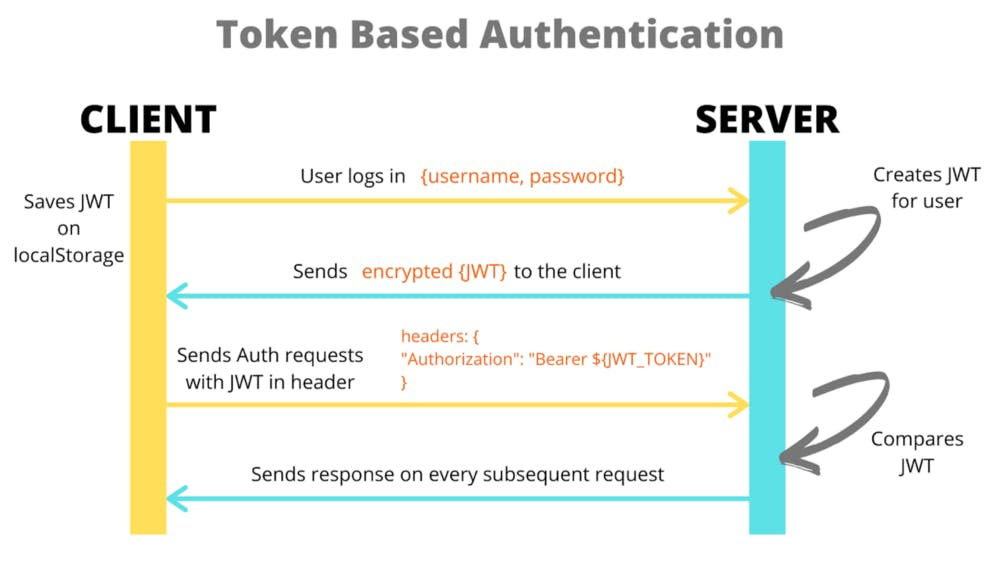
\includegraphics[scale=0.4]{JWT_authentication.jpg}
	\caption[{Λειτουργία JWT}]{Λειτουργία JWT \textbf{Πηγή:} \cite{fig_JWT_authentication}}
	\label{fig:JWT_authentication}
\end{figure}

\subsubsection{Δομή JWT}
Το ίδιο το token, το οποίο επιστρέφεται από το API, είναι απλώς μια κωδικοποιημένη συμβολοσειρά. Αποτελείται από τρία διαφορετικά τμήματα, τα οποία διαχωρίζονται μεταξύ τους με έναν χαρακτήρα τελείας. Αυτά είναι το header, το payload και το signature.

To header περιέχει δεδομένα σχετικά με τον τύπο του κουπονιού και τον αλγόριθμο που χρησιμοποιείται για τη δημιουργία του.

Το payload περιέχει δεδομένα σχετικά με το αίτημα και τον χρήστη που την υπέβαλε. Υπάρχει ένα σύνολο τυποποιημένων ζευγών κλειδιών/τιμών που ορίζονται ως μέρος του JWT, τα οποία μπορούν να χρησιμοποιηθούν:
\begin{itemize}
  \item Sub (Subject): Προσδιορίζει τον χρήστη που κάνει το αίτημα και πιστοποιείται.
  \item Iss (Issuer): Ο διακομιστής που εξέδωσε το token. Στην περίπτωσή μας, θα είχε νόημα να συμπεριλάβουμε το URI που χρησιμοποιείται
  \item Aud (Audience): Παρέχει κάποια μορφή ταυτοποίησης του παραλήπτη αυτού του κουπονιού.
  \item Exp (Ημερομηνία λήξης): Τα κουπόνια συνήθως δεν διαρκούν για πάντα. Η Exp εξασφαλίζει ότι όποιος χρησιμοποιεί το token παρέχει ένα πρόσφατα δημιουργημένο token.
\end{itemize}
Επίσης, είναι δυνατόν να καθοριστούν επιπρόσθετα ζεύγη κλειδιών/τιμών για την κάλυψη των αναγκών της υλοποίησης.

Τέλος, το signature είναι απλώς μια κωδικοποιημένη συμβολοσειρά που χρησιμοποιείται τόσο από τον διακομιστή όσο και από τον πελάτη για την επαλήθευση της αυθεντικότητας του payload.

Η αποκωδικοποιημένη δομή ενός παραδείγματος JWT token απεικονίζεται στο σχήμα \ref{fig:JWT_structure}.

\begin{figure}[h]
	\centering
	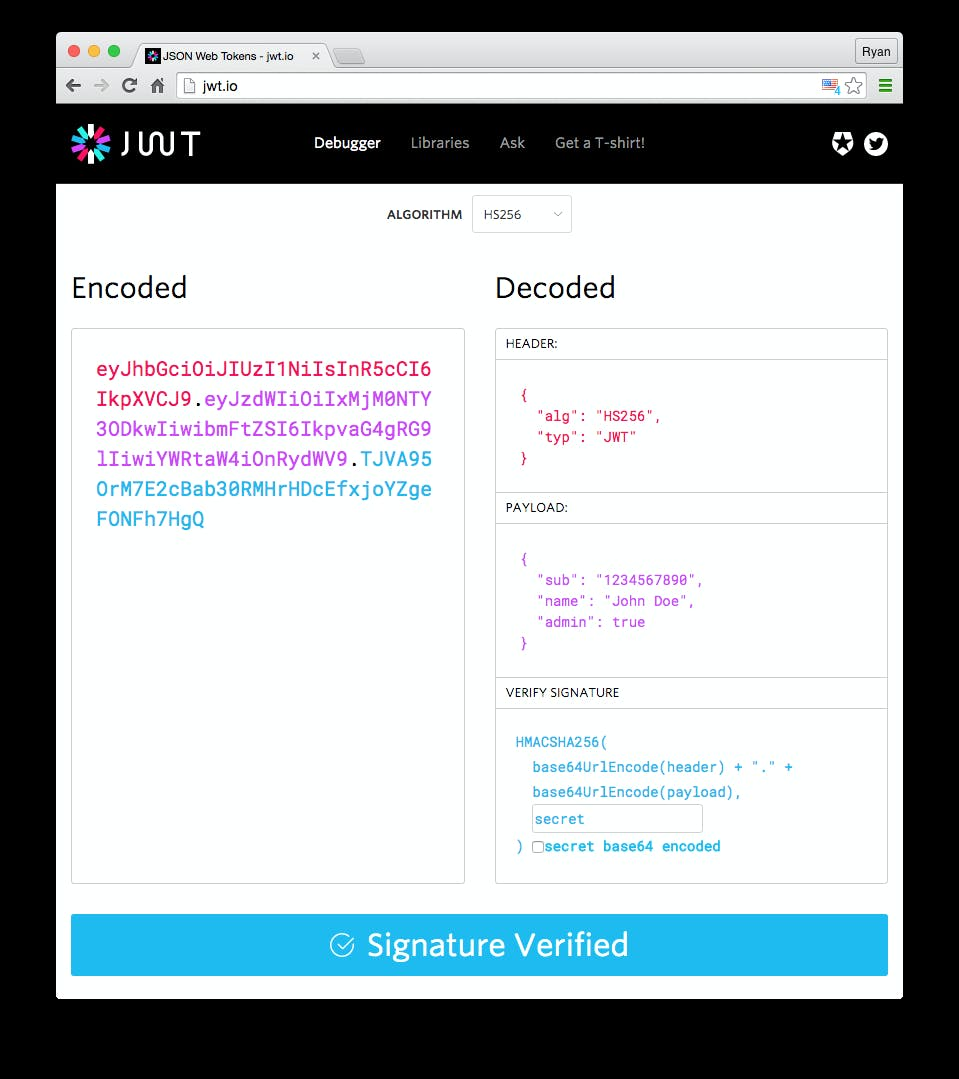
\includegraphics[scale=0.4]{JWT_structure.jpg}
	\caption[{Δομή JWT}]{Δομή JWT \textbf{Πηγή:} \cite{fig_JWT_structure}}
	\label{fig:JWT_structure}
\end{figure}

\subsection{Αντιμετώπιση SQL Injections}
\subsubsection{Τι είναι SQL Injection;}
Οι επιθέσεις τύπου SQL Injection προσπαθούν να εκμεταλλευτούν μια ευπάθεια στην ασφάλεια μιας διαδικτυακής εφαρμογής, η οποία επιτρέπει σε έναν εισβολέα να παρεμβαίνει στα ερωτήματα που κάνει η εφαρμογή στη βάση δεδομένων της. Αν υπάρχει ευπάθεια και ο εισβολέας καταφέρει να την εκμεταλλευτεί, μπορεί να αποκτήσει πρόσβαση σε δεδομένα που κανονικά δεν θα έπρεπε να είναι σε θέση να ανακτήσει ή ακόμη και να προκαλέσει καταστροφή της βάσης και απώλεια δεδομένων. Η αντιμετώπιση τέτοιων ευπαθειών είναι μείζονος σημασίας στις διαδικτυακές εφαρμογές, αφού οι επιθέσεις SQL Injection αποτελούν έναν από τους πιο διαδεδομένους τρόπους επίθεσης, είτε από μόνες τους, είτε σε συνδυασμό με άλλου τύπου επιθέσεις όπως DDoS attacks, DNS hijacking και Cross-Site Scripting (XSS).

\subsubsection{Prepared SQL Statements}
Οι προμεταγλωττισμένες εντολές SQL βοηθούν στην αντιμετώπιση των επιθέσεων τύπου SQL Injection. Με τη χρήση προμεταγλωττισμένων εντολών, οι τιμές των μεταβλητών που λαμβάνονται από τον χρήστη, αφού περάσουν από φίλτρο αντικατάστασης χαρακτήρων με ειδική σημασία στην SQL, ενσωματώνονται στην προμεταγλωττισμένη εντολή για να συνθέσουν το τελικό query που θα εκτελεστεί στη βάση δεδομένων. Έτσι, ενδεχόμενες κακόβουλες υποβολές τιμών από χρήστες, δε φτάνουν στο να εκτελεστούν στη βάση δεδομένων και να προκαλέσουν απώλεια ή υποκλοπή πληροφοριών.

\subsubsection{Ληφθέντα μέτρα αντιμετώπισης SQL Injections}
Η κλάση Query Builder του CodeIgniter4 \cite{CodeIgniter_querybuilder} έχει χρησιμοποιηθεί για την επικοινωνία της εφαρμογής με τη βάση δεδομένων της. Οι συναρτήσεις, που παρέχονται από τη συγκεκριμένη κλάση, καλούνται διαδοχικά και κάθε μια, με την εκτέλεσή της, προσθέτει από μια παράμετρο ώστε να συντεθεί το τελικό SQL Query προς εκτέλεση. Δέχονται ως ορίσματα τις απαραίτητες μεταβλητές, στις οποίες πραγματοποιούν αυτόματα την αντικατάσταση των ειδικών χαρακτήρων. Όταν κληθεί μια συνάρτησης ανάκτησης πληροφορίας από τη βάση, οι μεταβλητές ενσωματώνονται στο prepared query που έχει συνθέσει η κλήση των προηγούμενων συναρτήσεων, το ερώτημα εκτελείται και επιστρέφεται το αποτέλεσμα.

Για επιπρόσθετη ασφάλεια, καθώς η αντικατάσταση ειδικών χαρακτήρων δεν επαρκεί από μόνη της, αλλά και για κανονικοποίηση και επαλήθευση των τιμών των μεταβλητών του κάθε Μοντέλου, πριν ακόμη αυτές εισαχθούν στη βάση δεδομένων, έχει χρησιμοποιηθεί επίσης η βιβλιοθήκη Validation \cite{CodeIgniter_validation}. Στο κάθε Μοντέλο διατηρείται ένας πίνακας, ο οποίος περιέχει τα απαραίτητα φίλτρα επαλήθευσης για την κάθε τιμή μεταβλητής που δόθηκε από τον χρήστη ως είσοδος. Ο έλεγχος πραγματοποιείται πριν την εισαγωγή των δεδομένων στη βάση, η οποία πραγματοποιείται μόνο αν επικυρωθεί ότι οι τιμές που εξετάζονται είναι στη σωστή μορφή και τύπο.

Για παράδειγμα, έχει οριστεί ότι το αναγνωριστικό (ID) κάθε γραμμής ενός πίνακα, είναι ένας θετικός ακέραιος αριθμός. Αν ο χρήστης δοκιμάσει να εισάγει ως αναγνωριστικό κάποια είσοδο που δεν ικανοποιεί τον παραπάνω κανόνα, όπως κάποιο χαρακτήρα, η είσοδος θα απορριφθεί κατά τον έλεγχο εγκυρότητάς της. Ομοίως, δε θα γίνει αποδεκτή η είσοδος, αν στο πεδίο του email δεν είναι έγκυρο email ή αν το email που δόθηκε υπάρχει ήδη στον πίνακα, αφού έχει οριστεί και ως μοναδικό.

Ο συνδυασμός των παραπάνω πρακτικών, δηλαδή του ελέγχου εγκυρότητας των εισόδων και της ενσωμάτωσής τους σε prepared SQL statements, αποτελεί μια πολύ ισχυρή άμυνα ενάντια σε επιθέσεις τύπου SQL Injection.

\section{Σύνοψη Κεφαλαίου 4}
Στο κεφάλαιο 4, εξετάστηκαν όλες οι δυνατότητες της διαδικτυακής εφαρμογής και τα βήματα που πρέπει να ακολουθήσει ένας νέος χρήστης για να τις χρησιμοποιήσει. Επιπλέον, παρασχέθηκε οπτικό υλικό για κάθε λειτουργία στην οποία εμφανιζόταν στον χρήστη η διεπαφή χρήστη της διαδικτυακής εφαρμογής κατά την πλοήγησή του. Στη συνέχεια, εξηγήθηκαν διεξοδικά τόσο το front-end όσο και το back-end της δομής του πληροφοριακού συστήματος. Προκειμένου να διασφαλιστεί η ασφάλεια κατά τη χρήση της διαδικτυακής εφαρμογής, παρέχεται επεξήγηση των πρωτοκόλλων και των προσεγγίσεων ασφαλείας.

Στο επόμενο κεφάλαιο θα γίνει αξιολόγηση του συστήματος, ως προς την ορθή λειτουργία του και τις δυνατότητες κλιμάκωσής του.
